\documentclass[a4paper,12pt]{report}
\usepackage{stmaryrd}
\usepackage{ae}
\usepackage{aeguill}
\usepackage{amsthm}
\usepackage{eqnarray}
\usepackage[utf8]{inputenc}
\usepackage[T1]{fontenc}
\usepackage[french]{babel}
\usepackage{graphicx}
\usepackage{hyperref}
\usepackage{amssymb}
\usepackage{xcolor}
\usepackage[left=1cm, right=1cm, top=2cm, bottom=2cm]{geometry}
\usepackage{array,multirow}
\usepackage{amsmath,amsthm,amssymb}
\usepackage{amsfonts}
\usepackage{stmaryrd}
\usepackage{tcolorbox}
\usepackage{lmodern}
\usepackage{esint}
\usepackage[svgnames]{xcolor}
\usepackage{titlesec}

\setcounter{tocdepth}{1}

\newcommand{\Def}[2]{\begin{tcolorbox}[colback=white,colframe=CornflowerBlue, title=Définition : #1]#2\end{tcolorbox}}
\newcommand{\Thm}[2]{\begin{tcolorbox}[colback=white,colframe=Red!60, title=Théorème : #1]#2\end{tcolorbox}}
\newcommand{\Preuve}[2]{\begin{tcolorbox}[colback=white, title=Preuve: #1]#2\end{tcolorbox}}
\newcommand{\Methode}[2]{\begin{tcolorbox}[colback=white, title=Méthode :  #1]#2\end{tcolorbox}}

\newtheorem{Exe}{Exemple}[section]
\newtheorem{Exes}{Exemples}[section]
\newtheorem{Rem}{Remarque}[section]
\newtheorem{Rems}{Remarques}[section]

\def\R{\mathbb{R}}
\def\D{\mathbb{D}}
\def\C{\mathbb{C}}
\def\Q{\mathbb{Q}}
\def\N{\mathbb{N}}
\def\Z{\mathbb{Z}}
\def\K{\mathbb{K}}

\newcommand{\ind}{\perp\!\!\!\!\perp} 
\newcommand{\Rot}{\overrightarrow{\mathrm{rot}}}
\newcommand{\Grad}{\overrightarrow{\mathrm{grad}}}
\newcommand{\Div}{\mathrm{div}}
\renewcommand{\Vec}[1]{\overrightarrow{#1}}
\newcommand{\Phyvex}[3]{\left\vert\begin{matrix}#1\\#2\\#3\end{matrix}\right.}

\newcommand{\dx}{\mathrm{d}x}
\newcommand{\dt}{\mathrm{d}t}
\newcommand{\tr}{\mathrm{tr}}
\newcommand{\ev}{espace vectoriel}
\newcommand{\sev}{sous espace vectoriel}
\newcommand{\eve}{espace vectoriel euclidien}
\newcommand{\ssev}{\underset{\mathrm{sev}}{\subset}}
\newcommand{\ssgp}{sous groupe de}

\newcommand{\sce}{système complet d'évènements}
\newcommand{\ph}{\varphi}
\newcommand{\eps}{\varepsilon}
\newcommand{\som}[2]{\overset{#2}{\underset{#1}{\sum}}}
\newcommand{\produit}[2]{\overset{#2}{\underset{#1}{\prod}}}
\newcommand{\limit}[1]{\underset{#1}{\rightarrow}}
\newcommand{\eq}[1]{\underset{#1}{\sim}}
\newcommand{\inv}[1]{\frac{1}{#1}}
\newcommand{\acc}[1]{\left\{ #1 \right\}}
\newcommand{\mat}[2]{\left\{\[ \left( \begin{array}{#1} #2 \end{array} \right)\]}
\newcommand{\matv}[1]{\mathrm{Mat}_{\mathcal{#1}}}
\newcommand{\matf}[2]{\mathrm{Mat}_{\mathcal{#1,#2}}}
\newcommand{\scal}[1]{\langle #1 \rangle}
\newcommand{\norm}[1]{\lVert #1 \rVert}
\newcommand{\ssi}{\Longleftrightarrow}
\newcommand{\normt}[1]{{\left\vert\kern-0.25ex\left\vert\kern-0.25ex\left\vert #1 
    \right\vert\kern-0.25ex\right\vert\kern-0.25ex\right\vert}}
\newcommand{\leftaccolade}[1]{\left\{\begin{array}{l}#1\end{array}\right.}
\newcommand{\rightaccolade}[1]{\left.\begin{array}{l}#1\end{array}\right\} }
\DeclareMathOperator{\card}{card}
\newcommand{\sectionbreak}{\clearpage}


\renewcommand{\thechapter}{\Roman{chapter}}
\renewcommand{\thesection}{\Roman{section}}
\renewcommand{\thesubsection}{\Roman{section}.\arabic{subsection}}
\renewcommand{\thesubsubsection}{\Roman{section}.\arabic{subsection}.\Alph{subsubsection}}


\titleformat{\chapter}[block]
  {\normalfont\LARGE\bfseries}
  {\thechapter.}{1em}{}




\begin{document}

\tableofcontents
\renewcommand{\labelitemi}{$\cdot$}

\chapter{Analyse}
\section{Inégalités}

\Thm{Inégalité triangulaire}{ 
\textit{Pour:}
\begin{itemize}
  \item[] \(x,y \in\C\)
\end{itemize}
\textit{On a:}
\begin{itemize}
  \item[] \[||x|-|y||\leq|x+y|\leq|x|+|y|\]
\end{itemize}
}
\Thm{Inégalité de Cauchy-Schwartz (+ cas d'égalité)}{
\begin{itemize}
  \item[] \[ | \langle x, y \rangle | \leq \|x\| \cdot \|y\| \]
  \item[] \[ | \sum_{i=1}^n a_ib_i | \leq \sqrt{\sum_{i=1}^n a_i ^2 } \cdot \sqrt{\sum_{i=1}^n b_i ^2 } \]
  \item[] \[ | \int_{a}^b f(t) g(t) \dt | \leq \sqrt{\int_{a}^b f ^2 } \cdot \sqrt{\int_{a}^b g^2 } \]
  \textit{Il y a égalité si $x$ et $y$ sont colinéaire}
\end{itemize}
}
\Thm{Inégalité des accroissements finis}{
\textit{Pour:}
\begin{itemize}
  \item[] \(f : [a,b] \to \mathbb{R}\) continue sur \([a,b]\) 
  \item[] \(f\) dérivable sur \(]a,b[\)
\end{itemize}
\textit{On a:}
\begin{itemize}
  \item[] \[\forall x, y \in ]a, b[\ : |f(y)-f(x)|\leq \sup_{t \in ]a,b[} |f'(t)|\cdot |y-x| \]
\end{itemize}
}

\Thm{Inégalité de Jensen}{
  \textit{Pour:}
  \begin{itemize}
    \item[] \(f\) convexe sur \(I\) (intervalle)
    \item[] \(x_1,\dots,x_n\in I\)
    \item[] \(\lambda_1,\dots,\lambda_n\in[0,1]\) tq \(\sum_{i=1}^n \lambda_i=1\)    
  \end{itemize}
  \textit{On a:}
  \begin{itemize}
    \item[]\[\forall n\geq 2 : f\left(\sum_{i=1}^n \lambda_i x_i\right)\leq \sum_{i=1}^n \lambda_i f(x_i)\]
  \end{itemize}
}

\Thm{Petites inégalités}{
  \begin{center}
    \item[] \(\forall x>0: e^x > 1+x\)
    \item[] \(\forall x>-1: \ln(1+x) \leq x\)
    \item[] \(\forall x\in\R: |\sin(x)|\leq |x|\)
    \item[] \(\forall x\in [0,\frac{\pi}{2}]: \sin(x) \geq \frac{2}{\pi}x\)
    \item[] \(\forall (a,b)\in\R^2: |ab|\le\frac{a^2+b^2}{2}\)
    \item[] \(\forall x\in[0,1] x(1-x) \leq \frac{1}{4}\)
  \end{center}
}

\Thm{Inégalité arithmético-géométrique}{
  \textit{Pour:}
  \begin{itemize}
    \item[] \(a_1, a_2, \dots, a_n \geq 0\)
  \end{itemize}
  \textit{On a:}
  \begin{itemize}
    \item[] \[ \frac{a_1 + a_2 + \cdots + a_n}{n} \geq \sqrt[n]{a_1 a_2 \cdots a_n} \]
  \end{itemize}
}

\Thm{Caractérisation séquentielle de $f$ ne tend pas vers 0}{
\[f \not\xrightarrow[x\to \infty]{}0  \ssi \exists\varepsilon>0, \forall n \in \N, \exists x_n\!>\!n : f(x_n)\ge \varepsilon\]
}

\section{Intégrales généralisées}
\Def{Convergence d'intégrale}{
\textit{Pour:}
\begin{itemize}
  \item[] \(f\) continue sur \([a,b[\)
\end{itemize}
\textit{On a :}
\begin{itemize}
  \item[] \[\int_a^b f \text{ converge} \ssi \int_a^x f \xrightarrow[x\to b^-]{} l \in \R \]
\end{itemize}
}

\Thm{Divergence grossière à l’infini (Démo à refaire)}{
\textit{Pour:}
\begin{itemize}
  \item[] \(f\) cpm sur \([a,+\infty[\)
\end{itemize}
\textit{On a :}
\begin{itemize}
  \item[] \[\lim_{t\to+\infty} f(t) \neq 0 \implies \int_a^{+\infty} f \text{ diverge}\]
\end{itemize}
}

\Thm{Reste d'une intégrale généralisée}{
\[\text{Si } \int_a^b f \text{ CV: } \int_x^b f(t)\dt \xrightarrow[x\to b^-]{}0\]
}

\Thm{Astuce pour le cas positif}{
\textit{Pour}:
\(f\ge 0\)
\[\int_a^{+\infty} f(t) dt \text{ CV} \ssi \Bigg( \int_a^{na} f(t)dt \Bigg)_{n\in\N} \text{est majorée}\]
\textit{Utile pour montrer des divergence d'intégrale qui ne converge pas absolument (avec Chasles)}
}

\Thm{Comparaison à termes positifs}{
\textit{Pour:}
\begin{itemize}
  \item[] \(f,g\in C_{pm}\) positives
  \item[] $g$ d’intégrale convergente sur $[a,b[$
\end{itemize}
\textit{On a :}
\begin{itemize}
  \item[] \[f \underset{b^-}{=} o(g) \implies \int_a^b f \text{ converge}\]
  \item[] \[f \leq g \implies \int_a^b f \text{ converge}\]
  \item[] \[f\eq{b^-}g \implies \int_a^b f\text{ de même nature que }\int_a^b g\]
\end{itemize}
}

\Thm{Changement de variable}{
\[\text{Il suffit de faire un changement de variable $C^1$, bijectif et strictement monotone}\]
}

\Thm{IPP}{
\textit{Pour:}
\begin{itemize}
  \item[] \(u,v\in C^1([a,b[,\C)\)
  \item[] Le crochet $uv$ est fini
\end{itemize}
\textit{On a :}
\begin{itemize}
   \item[] \[\int_a^b u'v = \Big[uv\Big]^b_a - \int^a_buv'\]
   \item[] \[\int_a^b u'v \text{ de même nature que } \int_a^b uv'\]
\end{itemize}
}

\Thm{CV absolue $\implies$ CV}{
     \[\text{Une intégrale absolument convergente converge (en dim finie).}\]
}

\Thm{Intégration des relations de comparaison}{
\textit{Pour:}
\begin{itemize}
  \item[] \(f,g\in C_{pm}\) positives
  \item[] $g$ d’intégrale convergente sur $[a,b[$
\end{itemize}
\textit{On a:}
\begin{itemize}
    \item[] Si \(f(x) \sim_{x \to b} g(x)\), alors \[
        \int_x^b f(t) \, \mathrm{d}t \sim_{x \to b} \int_x^b g(t) \, \mathrm{d}t.
    \]
    \item[] Si \(f(x) = o(g(x))\), alors \[
        \int_x^b f(t) \, \mathrm{d}t = o\left( \int_x^b g(t) \, \mathrm{d}t \right).
    \]
\end{itemize}
\textit{Sinon pour:} $g$ d’intégrale divergente
\begin{itemize}
    \item[] Si \(f(x) \sim_{x \to b} g(x)\), alors \[
        \int_a^x f(t) \, \mathrm{d}t \sim \int_a^x g(t) \, \mathrm{d}t.
    \]
    \item[] Si \(f(x) = o(g(x))\), alors \[
        \int_a^x f(t) \, \mathrm{d}t = o\left( \int_a^x g(t) \, \mathrm{d}t \right).
    \]
\end{itemize}
}

\Thm{Intégrales de références}{
\begin{center}
    \item[] \(\int_1^{+\infty} \frac{\mathrm{d}x}{x^\alpha}\) converge  \( \ssi \alpha > 1\)
    \item[] \(\int_0^1 \frac{\mathrm{d}x}{x^\alpha}\) converge \( \ssi \alpha < 1\)
    \item[] \(\int_0^{+\infty} e^{-ax} \, \mathrm{d}x\) converge  \( \ssi a > 0\)
\end{center}

}

\Thm{Intégrales de Bertrand + démo}{
\begin{center}
    \item[] \(\int_1^{+\infty} \frac{\mathrm{d}x}{x^\alpha |\ln(x)|^\beta}\) converge \( \ssi \alpha > 1\) ou \(\alpha = 1\) et \(\beta > 1\)
    \item[] \(\int_0^1 \frac{\mathrm{d}x}{x^\alpha |\ln(x)|^\beta}\) converge \( \ssi \alpha < 1\) ou \(\alpha = 1\) et \(\beta > 1\)
    \item[]
    \item[] $\alpha=1$ : \text{preuve par calcul de l'intégrale}
\end{center}
}


\section{Séries numériques}
\Thm{Condition nécessaire de convergence}{
\[\sum u_n \text{ converge} \implies u_n \rightarrow 0 \]
et donc:
\[u_n \rightarrow l\neq 0 \implies \sum u_n \text{ diverge }\]
}

\Thm{Lien série-suite}{
\[\sum (u_{n+1} - u_n) \text{ de même nature que } (u_n)\]
}

\Thm{Critères de comparaison }{
\textit{Pour:} \((u_n)\in\C^\N, (v_n) \in \R_{+}^\N\)\\
\textit{On a:}
\[\text{Si } u_n \leq v_n \text{ à pdcr alors: } \sum v_n \text{ cv}  \implies \sum u_n \text{ cv}\]
\[\text{Si } u_n = \mathrm{o}(v_n) \text{ alors: } \sum v_n \text{ cv} \implies \sum u_n \text{ cv}\]
\[\text{Si } u_n \sim v_n \text{ alors: } \sum v_n \text{ cv} \implies \sum u_n \text{ cv}\]
}

\Thm{Sommation des relations de comparaison}{
\textit{Pour:} \((u_n)\in\C^\N, (v_n) \in \R_{+}^\N\) tel que \(\sum v_n\) cv\\
\textit{On a:}
\[\text{Si } u_n = \mathrm{o}(v_n) \text{ alors: } \sum_{k=n}^{+\infty} v_k =o\bigg(\sum_{k=n}^{+\infty} u_k\bigg) \]
\[\text{Si } u_n \sim v_n \text{ alors: } \sum_{k=n}^{+\infty} v_k \sim \sum_{k=n}^{+\infty} u_k\]

\textit{Si \(\sum v_n\) dv : comparaison des sommes partielles}
}

\Thm{CV absolue $\implies$ CV}{
\[\text{Une série absolument convergente converge (en dimension finie)}\]
}
\Thm{Séries usuelles}{
\[
\text{Série de Riemann : } \sum \inv{n^\alpha}  \text{ cv} \ssi \alpha>1 \]
\[\text{Série géométrique : } \sum q^n \text{ cv} \ssi |q|<1\]
\[\text{Série exponentielle : } e^z = \sum_{k=0}^\infty \frac{z^n}{n!}\]
}

\Thm{Stirling}{
\[n! \sim \sqrt{2\pi n }\,\big(\frac{n}{e}\big)^n\]
}

\Thm{CSSA}{
\[\rightaccolade{
(u_n) \text{ positive}\\
(u_n) \text{ décroissante}\\
u_n \xrightarrow[n\to\infty]{}0
} \implies
\begin{array}{l}
 \sum (-1)^n u_n \text{ cv}\\
 \forall n \in \N: |R_n|\leq|u_{n+1}|\\
 R_n \text{ du signe du premier terme}
\end{array}
\]
}

\Thm{Théorème de Cesàro}{
\[\forall (u_n)\in\C^\N : u_n \rightarrow l \implies \frac{1}{n}\sum_{k=1}^nu_k \rightarrow l\]
}

\Thm{Produit de Cauchy (dans $\C^\N$)}{
\textit{Pour:}
\begin{itemize}
  \item[] \(c_n = \sum_{k=0}^n a_kb_{n-k}\) (pour $n\in\N$)
\end{itemize}
\textit{On a:}
\begin{itemize}
    \item[] \[\sum a_n \text{ et } \sum b_n \text{ ACV} \implies \sum c_n \text{ ACV}\]
    \item[] \[\sum_{n=0}^{+\infty}c_n = (\sum_{n=0}^{+\infty}a_n)(\sum_{n=0}^{+\infty}b_n) \]
\end{itemize}
}
\Thm{Transformation d'abel}{
    \[\text{Transformation d'abel de \(\sum a_nb_n\): il faut exprimer $a_n = A_n-A_{n-1} $ et calculer la somme partielle}\]
}
\Methode{Ce qu'il faut savoir faire}{
    \[
    \begin{array}{l}
         \text{Séries de Bertrand ($\alpha=1$ preuve par calcul d'intégrale, donc comparaison série intégrale)}\\
         \text{Trouver des équivalents par $u_{n+1}^\alpha-u_n^\alpha$ puis sommation des relations de comparaison}  \\
    \end{array}
    \]
}

\section{Familles sommables}
\subsection{Cas des familles de réels positifs}
\Def{Somme d'une famille de réels positifs}{
On note :
\[\sum_{i\in I}u_i = \sup_{\underset{J finie}{J\subset I}}\sum_{i\in J}u_i\]

Si \(\sum u_i < +\infty\) la famille est dite sommable
}

\Thm{Sommation par paquets (cas positif)}{
Soit $(u_{i,j})_{(i,j) \in I \times J}$ une famille de réels positifs.

\textit{Pas d'hypothèse sur $(u_i)_{i\in I}$}
\[\sum_{i\in I}u_i = \sum_{n=0}^{+\infty}\Big(\sum_{i\in I_n}u_i\Big)\]
\textit{Attention : $I_n$ doit être dénombrable}
}

\Thm{Fubini (cas positif)}{
Soit $(u_{i,j})_{(i,j) \in I \times J}$ une famille de réels positifs.

Alors, 
\[
\sum_{(i,j) \in I \times J} u_{i,j} = \sum_{i \in I} \sum_{j \in J} u_{i,j} = \sum_{j \in J} \sum_{i \in I} u_{i,j}.
\]
}

\subsection{Cas des familles de réels ou complexes}
\Def{Famille sommable (réels ou complexes)}{
    \[(u_i)_{i\in I} \text{ sommable} \ssi (|u_i|)_{i\in I} \text{ sommable}\]
}

\Thm{Sommation par paquets (cas complexe)}{
Soit $(u_{i,j})_{(i,j) \in I \times J}$ une famille de complexes.\\
\textit{Si la famille est sommable (au sens des familles de complexes)} :
\[\sum_{i\in I}u_i = \sum_{n=0}^{+\infty}\Big(\sum_{i\in I_n}u_i\Big)\]
}

\Thm{Fubini (cas complexe)}{
Soit $(u_{i,j})_{(i,j) \in I \times J}$ une famille de complexes.\\
\textit{Si la famille est sommable (au sens des familles de complexes)} :
\[
\sum_{(i,j) \in I \times J} u_{i,j} = \sum_{i \in I} \sum_{j \in J} u_{i,j} = \sum_{j \in J} \sum_{i \in I} u_{i,j}.
\]
}

\subsection{Autres résultats}
\Thm{Permutation de sommme}{
Si la série $\sum u_n$ CVA, pour toute permutation $\sigma$ de $\mathbb{N}$:
\[
\sum_{n=0}^{+\infty} u_{\sigma(n)} = \sum_{n=0}^{+\infty} u_n.
\]
}

\section{Suites et séries de fonctions}
\subsection{Suites de fonctions}
\Def{2 modes de convergence (Suites de fonctions)}{
\[(f_n) \text{ CVS vers $f$ sur $I$} \ssi \forall x \in I : f_n(x)\longrightarrow f(x)\]
\[(f_n) \text{ CVU vers $f$ sur $I$} \ssi \lVert f_n-f \rVert_\infty \longrightarrow 0\]
}

\Thm{CVU $\implies$ CVS}{
\[\text{La convergence uniforme de $(f_n)$ implique la convergence simple $(f_n)$}\]
}

\Methode{Etablir la convergence uniforme}{
\begin{enumerate}
    \item[] On commence par déterminer la limite simple $f$ 
    \item La bornes supérieure sur $I$ de $|f_n-f|$ s’obtient par
fois par simple étude de fonction. Il suffit dans ce
 cas de passer à la limite.
    \item Sinon on majore par une suite indépendante de $x$:
    \item[] \(\forall x \in I : |f_n(x)-f(x)|\leq M_n \longrightarrow 0\)
\end{enumerate}
}

\Methode{Etablir la non-convergence uniforme}{
\begin{enumerate}
    \item[] Plusieurs possibilités: 
    \item la non-convergence simple
    \item le non respect des théorèmes de continuité et de doubles limites
    \item l'existence d'une suite $(u_n)$ telle que:
    \item[] \(|f_n(u_n) - f(u_n)| \not\rightarrow 0\)
\end{enumerate}
}

\Thm{Continuité de la limite uniforme}{
\textit{Pour:}
\begin{itemize}
  \item[] \((f_n) \text{ CVU vers $f$ sur $I$} \)
\end{itemize}
\textit{On a :}
\begin{itemize}
    \item[] \[f_n \in C^0 \text{ sur }  I\implies f\in C^0 \text{ sur }  I\]
\end{itemize}
}

\Thm{Théorème de la double limite}{
\textit{Pour:}
\begin{itemize}
  \item[] \((f_n) \text{ CVU vers $f$ sur $I$} \)
\end{itemize}
\textit{On a :}
\begin{itemize}
    \item[] \[\lim_{n\to\infty} \lim_{x\to a} f_n(x) = \lim_{x\to a} \lim_{n\to\infty} f_n(x) \]
\end{itemize}
}

\Thm{Échange intégrale et limite entière \underline{sur un segment}}{
\textit{Pour:}
\begin{itemize}
  \item[] \((f_n) \text{ CVU vers $f$ sur $[a,b]$} \)
\end{itemize}
\textit{On a :}
\begin{itemize}
    \item[] \[\lim_{n\to\infty} \int_a^b f_n(x)dx = \int_a^b \lim_{n\to\infty} f_n(x)dx \]
\end{itemize}
}

\Thm{De la classe $C^1$}{
\textit{Pour:}
\begin{itemize}
    \item[] \(\forall n \in \N : f_n \in C^1 \) sur $I$
    \item[] \((f_n) \text{ CVS vers $f$ sur $I$} \)
    \item[] \((f_n') \text{ CVU vers $g$ sur (tout segment de) $I$} \)
\end{itemize}
\textit{On a :}
\begin{itemize}
    \item[] \[f\in C^1 \text{ sur } I \text{ et } f'=g\]
\end{itemize}
}

\Thm{De la classe $C^k$}{
\textit{Pour :}
\begin{itemize}
    \item[] \(\forall n \in \mathbb{N} : f_n \in C^k \text{ sur } I\)
    \item[] 
    \(
    \left\{
    \begin{aligned}
        & (f_n^{(0)}) \text{ converge simplement vers } f \text{ sur } I, \\
        & (f_n^{(1)}) \text{ converge simplement vers } f' \text{ sur } I, \\
        & \vdots \\
        & (f_n^{(k-1)}) \text{ converge simplement vers } f^{(k-1)} \text{ sur } I
    \end{aligned}
    \right.
    \)
    \item[] \((f_n^{(k)}) \text{ converge uniformément vers } g \text{ sur tout segment de } I\)
\end{itemize}

\textit{On a :}
\begin{itemize}
    \item[] \[f \in C^k \text{ sur } I \text{ et } f^{(k)} = g\]
\end{itemize}
}

\subsection{Séries de fonctions}

\Def{3 modes de convergence (Séries de fonctions)}{
\[\sum f_n \text{ CVS sur $I$} \ssi (x \longmapsto S_n(x) ) \text{ CVS sur $I$}\]
\[\sum f_n \text{ CVU sur $I$} \ssi  (x \longmapsto S_n(x) ) \text{ CVU sur $I$}\]
\[\sum f_n \text{ CVN sur $I$} \ssi \sum \lVert f_n \rVert_{\infty} \text{ CV}\]
}

\Thm{Convergence uniforme : meilleure approche avec TSSA}{
 \[\text{$\sum f_n$ CVU $\ssi$ $\sum f_n$ CVS et \underline{$R_n$ CVU vers 0.}}\]
}

\Thm{CVN $\implies$ CVU}{
\[\text{La convergence normale de $\sum f_n$ implique la convergence uniforme de $\sum f_n$}\]
}

\Thm{}{

Les théorèmes suivants : 
\begin{itemize}
\item[] Continuité de la limite uniforme
\item[] Théorème de la échange limite somme
\item[] Échange intégrale et somme \underline{sur un segment}
\item[] Théorème de la classe $C^1$
\item[] Théorème de la classe $C^k$
\end{itemize}
ont les mêmes hypothèses que les suites de fonctions (au détail : $f_n = x\longmapsto S_n(x)$ près)
}

\subsection{Approximations uniformes}
\Thm{Approximation uniforme (segment)}{
 Toute fonction continue par morceaux sur un segment est limite uniforme d’une suite de fonctions
 en escalier.
}

\Thm{de Weierstrass (segment)}{
 Toute fonction continue sur un segment est limite
 uniforme de fonctions polynomiales
}

\Methode{Ce qu'il faut savoir faire}{
    \(
    \begin{array}{l}
         \text{Etude de $\zeta$ de Riemann:}\\
         \text{La fonction $\zeta$ de Riemann est de classe $C^\infty$ sur son ensemble de définition}\\
         \text{La fonction $\zeta$ de Riemann tend vers 1 en $+\infty$}\\
         \text{La fonction $\zeta$ de Riemann tend vers $+\infty$ en $1^+$}\\
         \text{La fonction $\zeta$ de Riemann est équivalente à  $x\longmapsto\frac{1}{x-1}$ en $1$}\\
         \text{Lemme de Riemann-Lebesgue}
    \end{array}
    \)
}


\section{Séries entières}
\subsection{Cas général : dans $\C$}
\Thm{Lemme d'Abel}{
\textit{Pour:}
\begin{itemize}
  \item[] \(r>0\)
\end{itemize}
\textit{On a :}
\begin{itemize}
    \item[] \[(a_nr^n) \text{ bornée} \implies \forall |z|<r : \sum a_nz^n \text{ converge absolument}\]
\end{itemize}
\textit{Le rayon de convergence (noté R) est le plus grand $r$ tel que : $(a_nr^n) \text{ bornée}$}
}

\Thm{Implication du RCV sur la série}{
    \[|z|<R \implies \sum a_nz^n \text{ converge absolument}\]
    \[|z|>R \implies \sum a_nz^n \text{ diverge grossièrement}\]
    \[|z|=R \implies \text{rien (on ne sait pas) }\]
}

\Thm{Comparaison}{
\begin{itemize}
  \item[] \[|a_n| {=} o(|b_n|) \implies R_a \geq R_b\]
  \item[] \[|a_n| \leq |b_n| \text{ (à pdcr)} \implies R_a \geq R_b\]
  \item[] \[|a_n|\eq{}|b_n| \implies  R_a = R_b\]
\end{itemize}
}

\Methode{En pratique}{
On utilisera souvent la règle d'Alembert $(R=\frac{1}{l})$
}

\Thm{CVN de la série entière}{
Convergence normale sur tout $\overline{D}(0,r)$ inclus dans $D(0,RCV)$ 
}

\Thm{Continuité de la série entière}{
 La somme d'une série entière est continue sur son disque ouvert de convergence.\\
 \textit{Attention: on est pas sûr que la SE CVS sur le disque fermé donc continue sur le disque fermé}
}

\Thm{d'Abel radial}{
\textit{Pour:}
\begin{itemize}
  \item[] \(\sum a_nx^n\) continue (défini) sur $]-R, R[$
\end{itemize}
\textit{On a :}
\begin{itemize}
    \item[] \[\sum a_nR^n \text{ converge} \implies \text{\(\sum a_nx^n\) continue (défini) sur $]-R, R]$}\]
\end{itemize}
}


\subsection{Cas réel : dans $\R$}
\Thm{Unicité de la série entière}{
S’il existe $\varepsilon>0$ tq:
 \[\forall x\in ]-\varepsilon, \varepsilon[ :  \sum_{n=0}^{+\infty}a_nx^n=\sum_{n=0}^{+\infty}b_nx^n \]
 Alors : \[\forall n \in \N : a_n = b_n\]
}

\Thm{En pratique (seulement sur $\R$)}{
\begin{itemize}
\item[] La somme d'une série entière est $C^\infty$ sur $]-R,R[$
\item[] On peut dériver comme on veut sur $]-R,R[$
\item[] On peut primitiver comme on veut sur $]-R,R[$
\item[] Si $f$ admet un développement en série entière: 
\item[] $\rightarrow$ Il est \underline{unique} et est donné par $\sum_{k=0}^n \frac{f^{(k)}(0)}{n!} x^k$
\end{itemize}
}

\Methode{Détermination du DSE}{
\begin{itemize}
\item[] Utilisation des développement usuels
\item[] Dérivation et intégration terme à terme
\item[] Formule de Taylor avec reste intégral
\item[] Décomposition en élément simple
\item[] Utilisation d'une équation différentielle
\end{itemize}
}

\section{Intégration des suites et séries de fonctions et intégrales à paramètres}
\subsection{Échange limite-intégrale}
\Thm{de convergence dominée}{
\textit{Si:}
\begin{itemize}
  \item[] \( (f_n) \text{ CVS vers } f\ \underline{\text{sur } I}\)
  \item[] \( f \text{ et } \forall n \in \N : f_n \text{ sont continue (p.m.) sur I}\)
  \item[] Domination : \(\forall n \in \N: |f_n|\leq\varphi\) avec $\varphi$ intégrable sur I
\end{itemize}
\textit{alors :}
\begin{itemize}
    \item[] \[\text{$f_n$ et $f$ sont intégrable sur I}\]
    \item[] \[\lim_{n\to+\infty} \int_I f_n = \int_I f\]
\end{itemize}
}

\Thm{de convergence dominée (à paramètre continue)}{
\textit{Si:}
\begin{itemize}
  \item[] \( \forall t \in J : f_x(t)\xrightarrow[x\to a]{} f(t)\) \textit{(avec $a$ un point de l'extrémité de I)}
  \item[] \( f \text{ et } \forall x \in I : f_x \text{ sont continue (p.m.) sur J}\)
  \item[] Domination : \(\forall x \in I, \forall t \in J :|f_x(t)|\leq\varphi(t)\) avec $\varphi$ intégrable sur J
\end{itemize}
\textit{alors :}
\begin{itemize}
    \item[] \[\text{$f_x$ et $f$ sont intégrable sur J}\]
    \item[] \[\lim_{x\to a} \int_J f_x = \int_J f\]
\end{itemize}
\textit{N.B. On notera plutôt $f(x,t)$}
}

\subsection{Échange somme-intégrale}
\Thm{Intégration terme à terme (Dernière hyp. négligeable si $(f_n)$ positive) }{
\textit{Si:}
\begin{itemize}
  \item[] \( (\sum f_n) \text{ CVS vers } S \ \underline{\text{sur } I}\)
  \item[] \( S \text{ et } \forall n \in \N : f_n \text{ sont continue (p.m.) sur I}\)
  \item[] \( \sum \int_I |f_n| \) converge (et $f_n$ intégrable)
 \end{itemize}
\textit{alors :}
\begin{itemize}
    \item[] \( \sum_{n=0}^{+\infty} f_n \) est intégrable sur \( I \),
    \item[] \( \sum_{n=0}^{+\infty} \int_I f_n = \int_I \sum_{n=0}^{+\infty} f_n \).
\end{itemize}
}

\subsection{Dérivation et Continuité}

\Thm{Continuité sous l'intégrale}{
$A$ une partie d'un EVN de dim finie\\
$f$ à valeurs dans A\\
\textit{Si :}
\begin{itemize}
    \item[] \( \forall t \in J : x \mapsto f(x,t) \in C^0 \),
    \item[] \( \forall x \in I: t \mapsto f(x,t) \in C_{\text{pm}} \),
    \item[] Domination : \( \forall (x,t) \in I \times J : |f(x,t)| \leq \varphi(t) \) avec \( \varphi \) intégrable sur \( J \),
\end{itemize}
\textit{alors :}
\begin{itemize}
    \item[] \( x \mapsto \int_J f(x,t)\,dt \) est définie et continue sur \( I \).
\end{itemize}
\textit{(On peut très bien localiser la domination ici)}
}


\Thm{Dérivation (classe \( C^1 \) des intégrales à paramètres)}{
\textit{Si :}
\begin{itemize}
    \item[] \( \forall t \in J : x \mapsto f(x,t) \in C^1 \),
    \item[] \( \forall x \in I : t \mapsto f(x,t) \) est intégrable,
    \item[] \( \forall x \in I : t \mapsto \frac{\partial f}{\partial x}(x,t) \in C_{\text{pm}} \),
    \item[] Domination : \( \forall (x,t)\in I \times J : \left| \frac{\partial f}{\partial x}(x,t) \right| \leq \varphi(t) \), avec \( \varphi \in L^1(J) \),
\end{itemize}
\textit{alors :}
\begin{itemize}
    \item[] \[ x \mapsto \int_J f(x,t) \,dt \in C^1(I) \]
    \item[] \[ \frac{d}{dx} \int_J f(x,t)\,dt = \int_J \frac{\partial f}{\partial x}(x,t) \,dt \]
\end{itemize}
\textit{(On peut très bien localiser la domination ici)}
}


\Thm{Dérivation (classe \( C^k \) des intégrales à paramètres)}{
\textit{Si :}
\begin{itemize}
    \item[] \( \forall t \in J : x \mapsto f(x,t) \in C^k \),
    \item[] \( \forall i \in \{0, \ldots, k-1\}, \forall x \in I : t \mapsto \frac{\partial^i f}{\partial x^i}(x,t) \) est intégrable,
    \item[] \( \forall x \in I : t \mapsto \frac{\partial^k f}{\partial x^k}(x,t) \in C_{\text{pm}} \),
    \item[] Domination : \( \forall (x,t) \in I \times J : \left| \frac{\partial^k f}{\partial x^k}(x,t) \right| \leq \varphi(t) \), avec \( \varphi \in L^1(J) \),
\end{itemize}
\textit{alors :}
\begin{itemize}
    \item[] \[ x \mapsto \int_J f(x,t)\,dt \in C^k(I) \]
    \item[] 
    \[
    \frac{d^k}{dx^k} \int_J f(x,t)\,dt = \int_J \frac{\partial^k f}{\partial x^k}(x,t)\,dt.
    \]
\end{itemize}
\textit{(On peut très bien localiser la domination ici)}
}

\section{Fonctions vectorielles}

Pour \( f \) à valeurs dans \( E \), un espace vectoriel normé sur \( \R \) ou \( \C \).

(La dérivation fonctionne coordonnée par coordonnée)

\Thm{Caractérisation des fonctions constantes}{
Pour \(f \in D^1\):
\[ f = \text{constante} \ \Leftrightarrow\ \forall t \in I : f'(t) = 0 \]
}

\Thm{Inégalité des accroissements finis (IAF)}{
\textit{Si :}
\begin{itemize}
    \item[] \( f \in C^0(I, E) \),
    \item[] \( f \in D^1(\mathring{I}, E) \),
    \item[] \( \exists M \geq 0, \forall t \in \mathring{I} : \|f'(t)\| \leq M \),
\end{itemize}
\textit{alors :}
\[
\forall (a,b) \in \overset{\circ}{I}^2 : \|f(b) - f(a)\| \leq M |b - a|.
\]
}

\section{Ensembles dénombrables}
\Def{Ensemble dénombrable / au plus dénombrable}{
\begin{itemize}
    \item \(E \text{ est dénombrable si : }  E \cong \N\)
    \item \(E \text{ au plus dénombrable si : }  E \cong \N \text{ ou } E \text{ fini}\) 
\end{itemize}
}

\Thm{Caractérisation de "au plus dénombrable"}{
\begin{align*}
    E \text{ au plus dénombrable} 
    &\ssi E \cong A\subset\N\\
    &\ssi \exists\text{ surjection}:\N\to E\\
    &\ssi \exists\text{ injection}: E\to \N\\
\end{align*}
}

\Thm{Liste usuelle d'ensembles dénombrables}{
    \[\N, \N^*, \Z, \N^2, \Q\]

    \textit{Pour $\N^2: (p,q)\longmapsto2^p(2p+1)$ est Injective par unicité de la décomposition en nombre premier; est aussi Surjective par décomposition en nombre premier\\\\TOUJOURS penser à la densité de $\Q$ dans $\R$ pour montrer qu'un ensemble est dénombrable}
}

\Thm{Produit et Union : dénombrabilité}{
    \[\prod_{\text{fini}} den = den\]
    \[\bigcup_{\text{Au plus den}} \textit{Au plus den} = \textit{Au plus den} \]
}

\section{E.V.N.}
\subsubsection{Norme}
\Def{Norme}{
Une norme est une application \( N : E \to \mathbb{R} \) vérifiant :
\begin{itemize}
    \item \( \forall x \in E, \ N(x) \ge 0 \)
    \item \( \forall x \in E, \ N(x) = 0 \iff x = 0_E \)
    \item \( \forall \lambda \in \mathbb{K}, \forall x \in E, \ N(\lambda x) = |\lambda| \cdot N(x) \)
    \item \( \forall x, y \in E, \ N(x + y) \leq N(x) + N(y) \)
\end{itemize}
}
\Def{Normes équivalentes}{
\( N \) et \( N' \) sont équivalentes s'il existe \( \alpha, \beta > 0 \) tels que :

\[
\forall x \in E, \quad \alpha N(x) \leq N'(x) \leq \beta N(x)
\]
}

\Def{Boule ouverte - Boule fermée - Sphere}
{
\[\text{Boule ouverte}: B(x_0, r) = \{x\in E/ \|x-x_0\|<r\} \]
\[\text{Boule fermée}: B_f(x_0, r) = \{x\in E/ \|x-x_0\|\le r\} \]
\[\text{Sphere}: S(x_0, r) = \{x\in E/ \|x-x_0\|= r\} \]
\textit{Les boules sont convexes}
}

\Thm{Justification de la continuité de la norme}{
    \[x\longmapsto \|x\| \text{ est 1-lipschitzienne}\]
}

\Thm{Normes équivalentes en dimension finie}{
\centering En dimension finie, toutes les normes sont équivalentes
}

\Def{Convexité d'un ensemble}{
\[A\subset E \text{ convexe} \overset{def}{\ssi} \forall (a,b) \in A^2, \forall t \in [0,1] : ta+(1-t)b \in A\]
\textit{Les boules sont convexes}
}

\subsubsection{Adhérence et extractions}
\Thm{Propriétés sur les extractions}{
\textit{Pour:}
\begin{itemize}
  \item[] $\varphi, \psi$ extractions
\end{itemize}
\textit{On a :}
\begin{itemize}
    \item \(\forall n\in \N : \varphi(n)\ge n\)
    \item \(\varphi \text{ est par définition strictement croissante}\)
    \item \(\varphi\circ\psi \text{ est une extraction}\)
\end{itemize}
}

\Thm{Traduction avec extraction : $(u_n)\in\R^\N$ pas majorée}{
\[(u_n)\in\R^\N \text{ pas majorée} \ssi \exists \varphi \text{ extraction / } u_{\varphi(n)} \to +\infty\]
}

\Thm{Traduction avec extraction : $(u_n)\in\R^\N$ ne tend pas vers 0}{
\[(u_n)\in\R^\N \text{ ne tend pas vers 0} \ssi \forall\varepsilon >0,\exists \varphi \text{ extraction, } \forall n\in \N : |u_{\varphi(n)}|\geq \varepsilon\]
}

\Thm{de Bolzano Weierstrass dans ($\R$ ou $\C$)}{
\[\text{Toute suite bornée (réel ou complexe) admet une valeur d'adhérence}\]
}

\Thm{Caractérisation de l'adhérence d'une suite}{
\vspace{-5mm}
\begin{align*}
    a \in \mathrm{Adh}(x_n) 
    &\ssi \forall \varepsilon>0 : \big \{n\in \N/\|x_n -a \|\leq \varepsilon\big\} \text{ est infini}\\
    &\ssi \forall\varepsilon>0: \forall n\in\N,\exists p\!>\!n \: x_n\in B_f(a,\varepsilon) 
\end{align*}
}
\subsubsection{Algèbre}
\Def{Algèbre Normée}{
\((A,+,\times,\cdot\) est une $\K$-algèbre si:
\begin{itemize}
    \item \((A,+,\times)\) est un anneau
    \item \((A,+,\cdot)\) est un $\K$-\ev
    \item $\forall(\lambda,a,b)\in \K\times A^2 : \lambda\cdot(a\times b) = (\lambda\cdot a)\times b = a\times(\lambda\cdot b)$
\end{itemize}
}
\Def{Norme d'algèbre}{
Soit $A$ une algèbre muni d'une norme $\|.\|$ :
\[\text{$\|.\|$ norme d'algèbre $\ssi \forall a,b \in\!A: \|a\times b\|\leq \|a\|\cdot\|b\|$}\]
}


\section{Topologie}
\subsubsection{Généralités}
\Def{Point intérieur/ Point adhérent}{
\[x\in\mathring{A} \ssi \exists r>0, \, B(x,r)\subset A \]
\[x\in\overline{A} \ssi \forall r>0, \, B(x,r)\cap A \neq \emptyset\]
}

\Def{Ouvert/Fermé}{
\[\text{A ouvert} \ssi \text{E$\textbackslash$A est fermé}\ssi A = \overset{\circ}{A}\]
\[\text{A fermé} \ssi \text{E$\textbackslash$A est ouvert}\ssi A = \overline{A}\]
}

\Thm{$\mathring{A}/\overline{A}$ est le plus ...}{
\[\text{$\mathring{A}$ est le plus grand ouvert de A}\]
\[\text{$\overline{A}$ est le plus petit fermé de A}\]
}

\Thm{Intersections - Unions - Produits d'ouverts}{
    \[\bigcup_{\infty} \text{ ouverts} = \text{ouvert},\; \bigcap_{finie} \text{ouverts} = \text{ouvert},\; \prod_{finie} \text{ouverts} = \text{ouvert}\]
    \[\bigcup_{finie} \text{fermés} = \text{fermé},\; \bigcap_{\infty} \text{ fermés} = \text{fermé},\; \prod_{finie} \text{fermés} = \text{fermé}\]
}

\Def{Densité}{
    \[\text{A dense dans E} \ssi \overline{A} = E\]
}

\Thm{F sev de E ev de dim finie alors F est :}{
Soit $F$ un \sev de $E$ et $E$ de dimension finie.
\[F \text{ est fermé}\]
}

\Thm{Norme triple associé à une norme}{
Pour $u\in\mathcal{L}_C(E,F)$:
\[\normt{u} = \sup_{x\in E\textbackslash\{0\}} \frac{\|u(x)\|}{\|x\|} = \sup_{\|x\|=1}\|u(x)\| =\sup_{\|x\|\leq1}\|u(x)\|\]

\textit{C'est une norme d'algèbre : $\normt{v\circ u}\leq\normt{v}\cdot\normt{u}$}
}

\subsubsection{Caractérisations séquentielles}
\Thm{Caractérisations séquentielle d'un point adhérent}{
\vspace{-5mm}
\begin{align*}
    a \in \overline{A}
    &\iff \exists (x_n) \in A^{\mathbb{N}}, \quad x_n \xrightarrow[n \to +\infty]{} a
\end{align*}

\textit{Penser à inf et sup}
}

\Thm{Caractérisation séquentielle d'un fermé}{
\vspace{-5mm}
\begin{align*}
    A \text{ fermé} &\iff \forall(x_n) \in A^{\mathbb{N}}, \quad x_n \xrightarrow[n \to +\infty]{} l \implies l \in A
\end{align*}
}

\Thm{Caractérisation séquentielle de la densité}{
\[\text{A dense dans E} \ssi \text{Tout élément de \( E \) est la limite d’une suite de \( A \)}\]
}

\Methode{Exemples à connaitre}{
\begin{itemize}
    \item $\mathcal{GL}_n(\R)$ dense dans $\mathcal{M}_n(R)$
    \item $a$ point isolé de $A$ $\ssi \exists\varepsilon\!>\!0 \, B(a,\varepsilon)\cap A = {a}$ 
    \item $a$ point d'accumulation de $A$ $\ssi \forall\varepsilon\!>\!0 \, B(a,\varepsilon)\textbackslash\{a\}\cap A \neq \emptyset$ 
\end{itemize}
}

\subsubsection{Continuité}

\Thm{Raisonnement par densité}{
\textit{Pour}:
\begin{itemize}
  \item[] $f,g$ continues sur E
  \item[] $A$ dense dans $E$
\end{itemize}
\textit{Alors}:
\[\text{$f$ et $g$ égales sur $A$ $\implies$ $f$ et $g$ égales sur $E$}\]
}

\Thm{Images réciproques}{
Pour $f$ continue:
\[\forall O \text{ ouvert}: f^{-1}(O) \text{ est ouvert}\]
\[\forall F \text{ fermé}: f^{-1}(F) \text{ est fermé}\]

\textit{C'est une double équivalence mais je préfère écrire ce côté de l'implication}
}

\Thm{f lipschitzienne $\implies$ ?}{
\[f \text{ lipschitzienne} \implies f \text{ uniformément continue}\]
}

\subsubsection{Continuité des applications linéaires et multi-linéaires}

\Thm{Caractérisations (4) de la continuité (applications linéaires)}{
\vspace{-5mm}
\begin{align*}
    f  \text{ linéaire est continue} 
    &\ssi f \text{ est lipschitzienne}\\
    &\ssi \forall\!x\!\in\!E: \|f(x)\|\leq C\|x\|\\
    &\ssi f\text{ bornée sur une boule de rayon $>0$}\\ 
    &\ssi f\text{ bornée sur la sphère unité}
\end{align*}
}

\Thm{Caractérisation de la continuité (applications multi-linéaires)}{
\vspace{-5mm}
\begin{align*}
    f  \text{ multi-linéaire est continue} 
    &\ssi \forall\!(x_i)_{i\in [|1,n|]}\!\in\! E_1 \times \dots \times E_n: \|f(x_1,\dots,x_n)\|\leq C\|x_1\|\dots\|x_n\|\\
\end{align*}
}

\Thm{Continuité et argument de dimension finie}{
\begin{itemize}
    \item f polynomiale : E dim finie $\implies$ f continue sur E
    \item f linéaire : E dim finie $\implies$ f continue sur E
    \item f multi-linéaire : \( E_1 \times \dots \times E_n \) de dimension finie $\implies$ f continue sur \( E_1 \times \dots \times E_n \).
\end{itemize}
}


\Methode{Homéomorphisme}{
\[\text{$f$ homéomorphisme $\ssi f\in C^0 , f$ bijective, $f^{-1} \in C^0$ 
}\]
}
\subsubsection{Compacité}
Dans tout ce paragraphe, le mot "compact" est remplacé par la lettre $\mathcal{K}_{pact}$
\Def{Partie compact}{
\( K\subset E \) est \(\mathcal{K}_{pact}\) ssi:
\begin{center}
    Toute suite de \( K \) admet une valeur d'adhérence dans \(K\)
\end{center}
}

\Thm{Fermée bornée}{
\begin{center}
     K un \(\mathcal{K}_{pact}\) de E$\implies$K \underline{fermé} et \underline{borné}
\end{center}
}

\Thm{Caractérisation des compacts en dim finie}{
Soit E de dim finie :
\begin{center}
     K un \(\mathcal{K}_{pact}\) de E $\ssi$ K \underline{fermé} et \underline{borné}
\end{center}
}

\Thm{Produit de compact}{
    \[\prod \mathcal{K}_{pact} = \mathcal{K}_{pact}\]
}

\Thm{Borne atteinte}{
Pour $f$ continue:
\[f(\mathcal{K}_{pact}) = \mathcal{K}_{pact}\]
\textit{Cas particulier si $f$ est à valeurs dans $\R$ : $f(\mathcal{K}_{pact})= [a,b]$}
}

\Thm{de Heine}{
\centering
$f\in C^0 \text{ sur } K \text{ un }\mathcal{K}_{pact} \implies f \text{ uniformément } C^0 \text{ sur } K$.
}

\Thm{de Bolzano Weierstrass}{
\[(u_n) \text{ bornée sur E de dim finie} \implies (u_n) \text{ admet une suite extraite convergente}\]
}

\subsubsection{Connexité par arcs}
\Def{Connexité par arc}{
\begin{center}
    \( A \) \textbf{connexe par arcs} $\ssi$ \(\forall a, b \in A \), \(\exists\gamma\) chemin reliant \( a \) à \( b \).
\end{center}
\textbf{Defintion d'un chemin :} Une application continue \( \gamma : [0,1] \to A \) avec \( \gamma(0) = a \) et \( \gamma(1) = b \).
}

\Thm{Image d'un connexe}{
Pour $f$ continue:
    \[f(\text{CPA}) = \text{CPA}\]
}

\Thm{TVI}{
Pour $f$ continue à valeurs dans $\R$:
    \[f(\text{CPA}) = \text{Intervalle}\]
}

\section{Calcul différentiel}
\textit{$\Omega$ désigne un ouvert de E (avec E de dimension finie) }
\subsubsection{Applications de classe $C^1$}
\Def{Différentielle en un point}{
Une application $f : \Omega \subset E \to F$ est dite différentiable en $a \in \Omega$ s'il existe $\varphi \in \mathcal{L}(E, F)$ tel que :
\[ f(a+h) \underset{h \to 0_E}{=} f(a) + \varphi(h) + o(\|h\|)\]
Si l'application $\varphi$ existe, elle est unique et est alors appelée \textit{différentielle} de $f$ au point $a$, on la note $\mathrm{d}f(a)$.
}

\Thm{Opération usuelles}{
\begin{itemize}
    \item \textbf{Linéarité :} $\mathrm{d}(\lambda f + \mu g)_a = \lambda \mathrm{d}f_a + \mu \mathrm{d}g_a$
    
    \item \textbf{Composition:} Si $f$ est différentiable en $a$ et $g$ en $f(a)$ :
    \[ \mathrm{d}(g \circ f)(a) = \mathrm{d}g({f(a)}) \cdot  \mathrm{d}f_a \]
\end{itemize}
}

\Thm{$f$ différentiable en a $\implies$ ?}{
\[f \text{ différentiable en a alors } f \in C^0 \text{ en a}\]
}

\Thm{Différentielle application multilinéaire}{
Soit $M : F^n \to \mathbb{R}$ une application multilinéaire et $f_1, \dots, f_n : E \to F$ différentiables en $a$. Pour tout $h \in E$ :
\[ \mathrm{d}(M(f_1, \dots, f_n))(a) \cdot h = \sum_{k=1}^n M\big(f_1(a), \dots, \mathrm{d}f_k(a) \cdot h, \dots, f_n(a)\big) \]
}

\Def{Dérivée selon un vecteur}{
Soit $f : \Omega \subset E \to F$ et $a, u \in E$. Si $t \mapsto f(a + tu)$ est dérivable en $0$, on appelle \textbf{dérivée de $f$ en $a$ selon $u$} la limite :
\[ D_u(f)(a) = \lim_{t \to 0} \frac{f(a + tu) - f(a)}{t} \]
}

\Thm{Lien dérivée selon un vecteur et différentielle}{
Si $f$ est différentiable en $a$, tout $u \in E$:
\[ D_u(f)(a) = \mathrm{d}f_a(u) \]
}

\Def{Dérivées partielles}{
Soit $f : \Omega \subset E \to F$ et $(e_1, \dots, e_p)$ une base de $E$. La \textbf{$j$-ième dérivée partielle} de $f$ en $a$ est la dérivée selon le vecteur $e_j$ :
\[ \frac{\partial f}{\partial x_j}(a) = D_{e_j}(f)(a) = \lim_{t \to 0} \frac{f(a + t e_j) - f(a)}{t} \]
}

\Thm{Calcul de la différentielle par dérivées partielles}{
Dans une base $B = (e_1,\dots,e_n)$
\[ df(a).h = \sum_{j=1}^p h_j \frac{\partial f}{\partial x_j}(a)\]
}

\Thm{Caractérisation de la classe $C^1$}{
\[f \in C^1 \ssi \forall j \in [\!|1,n|\!]: \frac{\partial f}{\partial x_j} \in C^0(\Omega)
 \ssi f  \text{ différentiable et } df\in C^0(\Omega)\]
}

\Def{Matrice Jacobienne}{
    \[
    J_f(x) = 
    \begin{pmatrix} 
    \frac{\partial f_i}{\partial x_j}
    \end{pmatrix}_{i,j\in\llbracket 1,n\rrbracket}
    \]

    \[
    J_{g \circ f}(x) = J_g(f(x)) \cdot J_f(x)
    \]
}

\Def{Gradient}{
\[df(a).h = (\nabla f(a) |h)\]
}

\Thm{Dérivation le long d'un arc}{
Pour \(\gamma : I\subset \R \to E\) et \(f : \Omega\to F \in C^1\) 
\[\forall t \in I, (f\circ\gamma)'(t) = df(\gamma(t)) .\gamma'(t)\]
}

\Thm{Intégration le long d'un arc}{
Soient $f$ et $\gamma : [0,1] \to \Omega$ de classe $C^1$. Si $\gamma(0)=a$ et $\gamma(1)=b$, alors :
\[ f(b) - f(a) = \int_{0}^{1} \mathrm{d}f_{\gamma(t)}(\gamma'(t)) \,\mathrm{d}t \]
}

\Thm{Caractérisation des fonctions constantes}{
Pour $\Omega$ un ouvert CPA et $f$ de classe $C^1$ sur $\Omega$. 
\[ f \text{ est constante sur }\Omega \iff \forall a \in \Omega, \mathrm{d}f_a = 0_{\mathcal{L}(E,F)} \]
}

\Def{Vecteur tangent}{
\[v\!\in\!E \text{ tangents à $X$ en } x \overset{def}{\ssi} \exists \varepsilon>0 , \exists \gamma \text{ arc dérivable en 0 tq:}\]
\[ \gamma\!:]-\varepsilon, \varepsilon[ \to X \text{ et } \gamma(0) =x \text{ et } \gamma'(0) = v\]
}

\Def{Hyperplan tangent à une ligne de niveau de f en x}{
Pour $f\in C^1$ et $df(x)\ne 0$, $X=\{x\in \Omega/f(x)=0\}$:
\[TxX = \ker(df(x)) =\nabla f(x)^\perp\]
}

\Thm{Dérivation composée ($\R^2$)}{
\[
F :
\begin{cases}
\mathbb{R}^2 \to \mathbb{R} \\
(x,y) \mapsto f(\varphi(x,y), \psi(x,y))
\end{cases}
\]

\[
\frac{\partial F}{\partial x}(x,y) =
\frac{\partial \varphi}{\partial x}(x,y) \cdot \frac{\partial f}{\partial x}(\varphi(x,y), \psi(x,y))
+ \frac{\partial \psi}{\partial x}(x,y) \cdot \frac{\partial f}{\partial y}(\varphi(x,y), \psi(x,y))
\]

\[
\frac{\partial F}{\partial y}(x,y) =
\frac{\partial \varphi}{\partial y}(x,y) \cdot \frac{\partial f}{\partial x}(\varphi(x,y), \psi(x,y))
+ \frac{\partial \psi}{\partial y}(x,y) \cdot \frac{\partial f}{\partial y}(\varphi(x,y), \psi(x,y))
\]

}





\Thm{$f(b)-f(a)$ et majoration}{
\[f(b)-f(a) = \int_0^1 df( \small{(1-t)a +tb}).(b-a) dt\]
\[\|f(b)-f(a)\|\le\sup_{t\in[0,1]}|\!\|df(tb+(1-t)a)\|\! |\,\|b-a\|\]
}

\subsubsection{Applications de classe $C^k$}

\Thm{de Schwarz}{
Si $f$ est de classe $C^2$ sur \textbf{un ouvert} $\Omega$, alors les dérivées partielles secondes croisées sont égales :
\[ \forall x \in \Omega, \quad \frac{\partial^2 f}{\partial x_i \partial x_j}(x) = \frac{\partial^2 f}{\partial x_j \partial x_i}(x) \]
}

\Def{Matrice Hessienne}{
Pour une fonction $f : \Omega \subset \mathbb{R}^n \to \mathbb{R}$ de classe $C^2$, la \textbf{hessienne} au point $a$ est la matrice symétrique :
\[ H_f(a) = \left( \frac{\partial^2 f}{\partial x_i \partial x_j}(a) \right) = 
\begin{pmatrix} 
\frac{\partial^2 f}{\partial x_1^2}(a) & \dots & \frac{\partial^2 f}{\partial x_1 \partial x_n}(a) \\
\vdots & \ddots & \vdots \\
\frac{\partial^2 f}{\partial x_n \partial x_1}(a) & \dots & \frac{\partial^2 f}{\partial x_n^2}(a)
\end{pmatrix} \in S_n(\mathbb{R}) \]
}

\Thm{Taylor-Young à l'ordre 2}{
Si $f$ est $C^2$ sur $\R^n$:
\[f(a+h) = f(a) + df(a) + \frac{1}{2} h^T H_f(a)h + o(\|h\|^2)\]
}

\Thm{Application polynomiale $\implies$ ?}{
\centering{Toutes les applications polynomiales sont $C^\infty$}\\
\textit{Car en calcul différentiel $E$ est de dimension finie}
}

\subsubsection{Optimisation}
\textit{Pour montrer l'existence d'un minimum penser au \textbf{Théorème des bornes atteintes} sur un compact}

\Def{Point critique}{
Soit $f$ de classe $C^1$ sur un \textbf{ouvert} $\Omega$. On dit que $a \in \Omega$ est un \textbf{point critique} de $f$ si :
\[ \mathrm{d}f_a = 0_{\mathcal{L}(E,\mathbb{R})} \quad \text{ou} \quad \nabla f(a) = 0 \]
}

\Thm{Condition nécéssaire d'existence d'un extremum}{
Soit $f : \Omega \subset E \to \mathbb{R}$ de classe $C^1$ sur un ouvert $\Omega$.
\[ f \text{ admet un extremum local en } a, \,\text{  alors } a \text{ est un point critique de } f \]
}

\Thm{Condition suffisante d'existence d'un minimum sur un ouvert}{
Soient $f : \Omega \subset E \to \mathbb{R}$ de classe $C^2$ sur l'ouvert $\Omega$ et $a \in \Omega$.
\begin{itemize}
    \item si $f$ atteint en $a$ un minimum local, $H_f(a) \in \mathcal{S}_n^+(\mathbb{R})$.
    \item si $a$ est un point critique de $f$ et si $H_f(a) \in \mathcal{S}_n^{++}(\mathbb{R})$, alors $f$ atteint en $a$ un minimum local.
\end{itemize}
}

\Thm{Corollaire CS extremum}{
Soient $f : \Omega \subset E \to \mathbb{R}$ de classe $C^2$ sur l'ouvert $\Omega$ et $a \in \Omega$ un point critique de $f$.
\begin{itemize}
    \item Si $\text{Sp}(H_f(a)) \subset \mathbb{R}_+^*$, $f$ atteint en $a$ un minimum.
    \item Si $\text{Sp}(H_f(a)) \subset \mathbb{R}_-^*$, $f$ atteint en $a$ un maximum.
    \item Si $H_f(a)$ possède deux valeurs propres de signes distincts, $a$ est un point selle.
\end{itemize}
}

\Thm{Optimisation sous contrainte}{
Soient $f, g$ de classe $C^1$ sur $\Omega$. On pose $X = \{x \in \Omega \mid g(x)=0\}$.\\
Si $f|_X$ admet un extremum local en $a \in X$ et $\mathrm{d}g(a) \neq 0$, alors :
\[ \exists \lambda \in \mathbb{R}, \quad \mathrm{d}f(a) = \lambda \mathrm{d}g(a) \]
}

\section{Équations différentielles}
\subsubsection{Équations linéaires scalaires d’ordres 1 et 2}

\Thm{Équation d'ordre 1}{
Si $a,b : I \to \mathbb{K}$ continues et $A$ une primitive de $a$ :
\begin{itemize}
    \item $(H): y'=a(t)y \Rightarrow y(t) = \lambda e^{A(t)}$
    \item $(E): y'=a(t)y+b(t) \Rightarrow y(t) = y_p(t) + \lambda e^{A(t)}$
\end{itemize}
}

\Thm{Problème de Cauchy (ordre 1)}{
Si $a$ ne s’annule pas sur $I$ :\\
\[
\left\{
\begin{aligned}
    a(t)y' + b(t)y &= c(t) \\
    y(t_0) &= y_0
\end{aligned}
\right.
\longrightarrow \text{unique solution sur } I
\]
}
\Thm{Structure des solutions (ordre 1)}{
Si $a$ ne s’annule pas sur $I$ :
\begin{itemize}
    \item $\mathcal{S}_H$ est un espace vectoriel
    \item $\mathcal{S}_E$ est une droite affine de direction $\mathcal{S}_H$
\end{itemize}
}

\Methode{Plan de résolution (ordre 1)}{
\begin{itemize}
    \item Identifier l’équation
    \item Diviser par $a(t)$ si possible
    \item Résolution de l’équation homogène
    \item Trouver une solution particulière (variation de la constante)
    \item Solution générale : $y = y_p + \lambda y_h$
    \item Recollement éventuel des solutions (souvent via un DL).
    \item Conditions initiales
\end{itemize}
}

\Thm{Problème de Cauchy (ordre 2)}{
Si $a$ ne s’annule pas sur $I$ :\\
\[
\left\{
\begin{aligned}
    a(t)y'' + b(t)y' + c(t)y &= d(t) \\
    y(t_0) = y_0,\quad y'(t_0) = y_0'
\end{aligned}
\right.
\longrightarrow \text{unique solution sur } I
\]
}

\Thm{Structure des solutions (ordre 2)}{
Si $a$ ne s’annule pas sur $I$ :
\begin{itemize}
    \item $\mathcal{S}_H$ est un plan vectoriel
    \item $\mathcal{S}_E$ est un plan affine de direction $\mathcal{S}_H$
\end{itemize}
}

\Thm{Principe de superposition}{
Si $y_1$, $y_2$ solutions de $y''+by'+cy=d_1$ et $d_2$, alors $y_1+y_2$ est solution pour $d_1+d_2$.
}

\Methode{Résolution avec coefficients constants}{
On résout l’équation caractéristique : $ar^2 + br + c = 0$\\
\begin{itemize}
    \item $\Delta > 0$: $y_h = \lambda_1 e^{r_1 t} + \lambda_2 e^{r_2 t}$
    \item $\Delta = 0$: $y_h = (\lambda_1 + \lambda_2 t)e^{r t}$
    \item $\Delta < 0$: $y_h = e^{\alpha t} (\lambda_1 \cos \beta t + \lambda_2 \sin \beta t)$
\end{itemize}
}

\Methode{Trouver une solution particulière (coeff. constants)}{
\begin{itemize}
    \item Si $d(t) = P(t)e^{mt}$, poser $y_p = Q(t)e^{mt}$
    \item Si $d(t) = \cos(\omega t)$ ou $\sin(\omega t)$, on passe en complexe
\end{itemize}
}

\Methode{Résolution avec coefficients non constants}{
(Suivre l’énoncé)
\begin{itemize} 
    \item Recherche de solutions polynomiales (commencer par l’étude du degré)
    \item Recherche de solutions développables en série entière
    \item Recherche sous la forme $y(t) = z(t)y_0(t)$, où $y_0$ est une solution connue 
    \item Changement de variables ou d’inconnues
\end{itemize}
}

\subsubsection{Systèmes différentiels linéaires}

\Thm{Cauchy linéaire}{
Soient $I$ un intervalle de $\mathbb{R}$, $t_0 \in I$ et $X_0 \in \mathcal{M}_{n,1}(\K)$.
Si $A : I \to \mathcal{M}_n(\K)$ et $B : I \to \mathcal{M}_{n,1}(\K)$ sont continues sur $I$,
alors le problème de Cauchy
\[
\begin{cases}
X' = AX + B \\
X(t_0) = X_0
\end{cases}
\]
admet une et une seule solution.
}

\Thm{Structure des solutions}{
Lorsque $A : I \to \mathcal{M}_n(\K)$ et $B : I \to K^n$ sont \textbf{continues} sur l’intervalle $I$,
\begin{itemize}
    \item l’ensemble $\mathcal{S}_H$ des solutions de $X' = A(t)X$ est un s.e.v. de $\mathcal{C}^1(I, \K^n)$ de dimension $n$ ;
    \item l’ensemble des solutions de $X' = A(t)X + B(t)$ est un s.e. affine de $\mathcal{C}^1(I, \K^n)$ de direction $\mathcal{S}_H$.
\end{itemize}
}

\Thm{Caractérisation du système fondamentale (sans wronskien)}{
Si on a:
\begin{itemize}
\item $t\mapsto A(t)$ continue sur $I$
\item $X_1, \dots, X_n$ des solutions du système $X' = A(t)X$
\end{itemize}
Alors, les assertions suivantes sont équivalentes :
\begin{enumerate}
    \item $(X_1, \dots, X_n)$ est un système fondamental de solutions ;
    \item pour tout $t \in I$, $(X_1(t), \dots, X_n(t))$ est une base de $\K^n$ ;
    \item il existe $t_0 \in I$ tel que $(X_1(t_0), \dots, X_n(t_0))$ soit une base de $\K^n$.
\end{enumerate}
}

\Methode{Transformation d'une équation différentielle linéaire d'ordre $n$ en une équation matricielle}{
$x^{(n)} = a_0(t)x + a_1(t)x' + \cdots + a_{n-1}(t)x^{(n-1)} \ssi X' = A(t)X$\\
où:
\[
X =
\begin{pmatrix}
x \\
x' \\
\vdots \\
x^{(n-1)}
\end{pmatrix}, \quad
A =
\begin{pmatrix}
0      & 1      & 0      & \cdots & 0      \\
0      & 0      & 1      & \cdots & 0      \\
\vdots & \vdots & \ddots & \ddots & \vdots \\
0      & 0      & \cdots & 0      & 1      \\
a_0   & a_1   & \cdots & \cdots & a_{n-1}
\end{pmatrix}
\]
}

\Def{Wronskien}{
On appelle wronskien d’une famille de solutions $(X_1, \dots, X_n)$ du système $X' = A(t)X$, l’application :
\[
W : t \mapsto \det\big(X_1(t), \dots, X_n(t)\big).
\]

\textbf{Pour n=2:}
Deux solutions $x_1$, $x_2$ de $x'' + b(t)x' + c(t)x = 0$, on pose :
\[
W = 
\begin{vmatrix}
x_1 & x_2 \\
x_1' & x_2'
\end{vmatrix}
\]
}

\Thm{Caractérisation d'un système fondamental avec le wronskien}{
\[
(X_1, \dots, X_n)\ \text{est un système fondamental}
\ \Longleftrightarrow\ 
\forall t \in I,\ W(t) \neq 0
\ \Longleftrightarrow\ 
\exists t_0 \in I,\ W(t_0) \neq 0.
\]
\hspace{1em}
}

\Methode{Variation des constantes}{
\textbf{Méthode de variation des constantes}

Soit le système :
\[
X' = A(t)X + B(t)
\]
et $(X_1, \dots, X_n)$ un système fondamental de solutions de l’équation homogène
\[
X' = A(t)X.
\]

\begin{itemize}
    \item Toute solution de l’équation homogène s’écrit :
    \[
    X_h(t) = \lambda_1 X_1(t) + \cdots + \lambda_n X_n(t).
    \]

    \item On cherche une solution particulière sous la forme :
    \[
    X(t) = \lambda_1(t) X_1(t) + \cdots + \lambda_n(t) X_n(t).
    \]

    \item En dérivant et en injectant dans l’équation :
    \[
    \lambda_1'(t) X_1(t) + \cdots + \lambda_n'(t) X_n(t) = B(t).
    \]
    \item On résout ce système
    \item La solution générale est alors :
    \[
    X(t) = \sum_{i=1}^n \lambda_i(t) X_i(t).
    \]
\end{itemize}
}
\subsubsection{Système différentiel linéaire à coefficients constants}

\Thm{Solution générale à coefficients constants}{
Soit $A \in \mathcal{M}_n(\K)$. L’équation homogène $X' = AX$ admet pour solution générale :\\
\[
X : t \mapsto e^{tA}C \quad \text{avec } C \in \K^n
\]
\textit{Penser à Cayley-Hamilton}
}

\Thm{Solution pour coefficients constants (cas diagonalisable) }{
Soit $A \in \mathcal{M}_n(\mathbb{C})$ une matrice diagonalisable. \\
Il existe alors une base $(V_1, \dots, V_n)$ de vecteurs propres associés aux valeurs propres $\lambda_1, \dots, \lambda_n$.

Les solutions de l’équation
\[
X' = AX
\]
sont de la forme :
\[
X(t) = c_1 e^{\lambda_1 t} V_1 + \cdots + c_n e^{\lambda_n t} V_n
\quad \text{avec} \quad c_1, \dots, c_n \in \mathbb{K}.
\]
}



\chapter{Algèbre}
\section{Complément d'algèbre linéaire}
\Thm{De la base incomplète}{
    Soit $\mathcal L$ une famille libre de $E$, alors:
    \[\mathcal L \text{ peut être compléter en une base de $E$}\]
}
\Thm{De la base extraite}{
    Soit $\mathcal G$ une famille génératrice de $E$, alors:
    \[\mathcal G \text{ peut être extraire en une base de $E$}\]
}
\Thm{Caractérisation des sommes directes}{
  Soient $F_1, \dots, F_p$ des espaces (ou sous-espaces). Ils forment une somme directe si
  \[
    \forall x_1, \dots, x_p \in \prod_{i=1}^p F_i, \quad \left( \sum_{i=1}^p x_i = 0 \right) \implies \left( \forall i,\, x_i = 0 \right).
  \]
}

\Thm{Propriété 2 polynômes d'endomorphisme}{
  Soit $v\in\mathcal{L}(E)$, $P,Q\in\K[X]$:
  \[(PQ)(u)=P(u)\circ Q(u)=Q(u)\circ P(u)\]
}

\Def{Projecteur spectral}{
  Si $E = \bigoplus_{i=1}^n E_{\lambda_i}(u)$ alors on a : \[\forall x \in E : x= x_1+...+x_n \quad(\text{où $x_i\in E_{\lambda_i}(u)$})\]
  On note alors $\pi_i : x\mapsto x_i$ la projection spectral sur $E_{\lambda_i}(u)$\\
  On a alors :
  \[ \pi_1+...+\pi_n = id_E \quad \forall i\neq j: \pi_i \circ \pi_j = 0_{\mathcal{L}(E)}\]
}

\section{Réduction d'endomorphismes}
\subsubsection{Généralités}

\Thm{Caractérisation matricielle de l'induit}{
\[
F \text{ stable par } u \ssi \text{mat}_{B}(u) = 
\begin{pmatrix}
A & B \\
0 & C
\end{pmatrix}
\]
\( A \) est la matrice de l'endomorphisme induit sur \( F \) (dans la base de $E$ restreint à une base de $F$)
}

\Thm{Matrice d'une somme directe}{
Soit $E = \bigoplus_{i=1}^p E_i$, B une base adaptée à la décomposition:

\[
\forall i : E_i \text{ stable par } u \ssi \text{mat}_{B}(u) = 
\begin{pmatrix}
A_1 & 0 &... &0 \\
0 & A_2 & ...&0 \\
\vdots & & \ddots & \vdots\\
0& \cdots & \cdots & A_n
\end{pmatrix}
\]
avec $A_i = \mathrm{mat}_{B_i}(E_i)$
}

\Def{Valeurs propres et espaces propres}{
\[ Sp(u) = \{ \lambda \in \mathbb{K} \ | \ \exists x \in E \setminus \{0_E\}, u(x) = \lambda x \} \]
\[ E_{\lambda_i}(u) = \ker (u - \lambda_i \operatorname{id}_E)=\K e_i\]

où $(e_1, ..., e_n)$ est une base de vecteurs propres\\
\textit{Matrice triangulaire supérieure: valeurs propres $\rightarrow$ sur la diagonale}
}

\Thm{Valeurs propres distinctes $\implies$ ?}{ 
     \centering Les sous-espaces propres associés à des valeurs propres distinctes sont en somme directe.\\
     Toute famille de vecteurs propres associés à des valeurs propres distinctes est libre.
}

\Thm{Transmission de la diagonalisation à l'induit}{
On a : $\chi_{u_{F}} | \chi_u$ \textit{(en écrivant $mat(u)$ dans une base adaptée)}\\
On a : $\pi_{u_{F}} | \pi_u$ \textit{(car $\pi_u(u_F) = 0$)}\\
Soit $u\in\mathcal{L}(E)$ diagonalisable, $F\subset E$ stable par $u$, on a:
\[
u_F \text{ diagonalisable}
\]

\textit{Preuve: polynôme minimal}
}


\subsubsection{Polynôme caractéristique}
\Def{Polynôme caractéristique}{
\[ \chi_M(X) = \det(X I_n - M) \]
\[ \forall B : \chi_u(X) = \det(X I_n - \mathrm{Mat}_B(u)) \]
}
\Thm{Polynôme caractéristique de 2 matrices semblabes}{
\[A \text{ semblable à } B \implies \chi_A = \chi_B\]
}

\Thm{Polynôme caractéristique d'une matrice triangulaire par bloc}{
\[\chi_A = \prod_{i=1}^p \chi_{A_i, blocs}\]

}

\Thm{Écriture en extension du polynôme caractéristique}{
\[\chi_u = X^n-tr(u)X^{n-1}+\cdots+(-1)^ndet(u)\]
}

\Thm{Inégalité de l'espace propre}{
\[1\leq \mathrm{dim} E_\lambda(u)\leq \mathrm{mult}(\lambda)\]
}

\subsubsection{Polynôme annulateur et minimal}
\Thm{Stabilité des espaces propres}{
\textit{Pour: }\(P\in \mathbb{K}[X]\)
\begin{itemize}
    \item[] \[\mathrm{Im}(P(u)) \text{ et } \mathrm{Ker}(P(u)) \text{ sont stable par u}\]
    \item[] \[\text{Si } v\circ u = u \circ v \text{ alors: } \mathrm{E}_\lambda(u) \text{ stable par $v$}\]
\end{itemize}
}

\Def{Polynôme annulateur et minimal}{
\[ P \text{ annulateur de } u \ssi P(u) =0\]
\[ \pi_u \text{ est l'unique polynôme unitaire qui divise tous les polynômes annulateurs de } u \]
}

\Thm{Polynôme annulateur de 2 matrices semblables}{
\[A \text{ semblable à } B \implies \pi_A = \pi_B\]
}

\subsubsection{Diagonalisation}
\Thm{Lien entre le spectre et les racines}{
\[\mathrm{Sp}(u)\subset\mathrm{Rac}(P \text{ annulateur})\]
\[\mathrm{Sp}(u)=\mathrm{Rac}(\pi_u)\]
\[\mathrm{Sp}(u)=\mathrm{Rac}(\chi_u)\] 
}
\Thm{CNS de diagonalisation}{
\begin{align*}
M \text{ diagonalisable}
    &\ssi E =\!\!\!\bigoplus_{\lambda\in Sp(M)}\!\!\!E_\lambda \quad \text{ ou } \quad \mathrm{dim}(E) =\!\!\!\sum_{\lambda\in Sp(M)}\!\!\!\mathrm{dim}(E_\lambda)\\
    &\ssi \chi_M \text{ scindé} \qquad \text{ et} \qquad  \text{dim($E_\lambda$)=mult($\lambda$)}\\
    &\ssi \exists P \text{ annulateur SARS}\\
    &\ssi \pi_M \text{ est SARS}\\
\end{align*}
}

\Thm{CN de diagonalisation}{
\begin{align*}
\chi_M \text{ SARS}
    &\implies M \text{ diagonalisable}\\
\end{align*}
}

\Thm{CNS de trigonalisation}{
\begin{align*}
M \text{ trigonalisable}
    &\ssi \chi_M \text{ scindé}\\
    &\ssi \pi_M \text{ scindé}\\
    &\ssi \exists P \text{ annulateur scindé}\\
\end{align*}
}

\subsubsection{Autres théorèmes}
\Thm{CNS nilpotence}{
\begin{align*}
M \text{ nilpotente}
    &\ssi \mathrm{Sp}(M) = \{0\} \text{ et $M$ trigonalisable} \\
    &\ssi \chi_M = X^n\\
\end{align*}
}

\Thm{Cayley Hamilton}{
\[\chi_M (M) = 0 = \chi_u(u)\]
}

\Thm{Décomposition des noyaux}{
\textit{Pour: }\(P=\prod_{i=1}^r P_i\) avec les $P_i$ 2 à 2 premiers entre eux
\[\ker P(u)=\bigoplus_{i=1}^r \ker P_i(u).\]
}

\section{Espace euclidien et préhilbertien}

\subsubsection{Rappels}
\Def{Produit scalaire}{

$\varphi : E\times E \to \R$ est un \textbf{produit scalaire} si : 
\vspace{0.5em}
\\
$\varphi$ est symétrique: $\forall x,y\in E : \varphi(x,y) = \varphi(y,x)$\\
$\varphi$ est bilinéaire: $\forall x,y,z\in E, \forall \lambda \in \R: \varphi(\lambda x+y,z) = \lambda\varphi(x,z)+\varphi(y,z)$\\
\textit{(idem pour l'autre variable)}\\
$\varphi$ est définie positive: $\forall x\in E : \varphi(x,x)\ge 0$ et $\varphi(x,x) = 0 \ssi x = 0_E$
}

\Thm{Identité de polarisation}{
\[
\langle x , y \rangle = \frac{1}{4}\left(\lVert x + y \rVert^2 - \lVert x - y \rVert^2\right).
\]
}

\Thm{Cauchy-Schwarz}{
Soit $(E, \langle \cdot | \cdot \rangle)$ un espace préhilbertien réel. Alors,
\begin{equation*}
    \forall x, y \in E, \quad |\langle x , y \rangle| \leqslant \|x\| \cdot \|y\|
\end{equation*}
Il y a égalité si et seulement si $x$ et $y$ sont colinéaires.
}

\Thm{Pythagore}{
Soient $x, y \in E$. \[ \|x + y\|^2 = \|x\|^2 + \|y\|^2 \iff \langle x , y \rangle = 0.\]
}

\Def{Familles orthogonales et orthonormales}{
(i) Une famille $(e_i)_{i \in I}$ quelconque de vecteurs de $E$ est dite orthogonale si :
\begin{equation*}
    \forall(i, j) \in I^2, \quad i \neq j \implies \langle e_i , e_j \rangle = 0.
\end{equation*}

(ii) Elle est dite orthonormale si elle vérifie de plus : \quad $\forall i \in I, \quad \|e_i\| = 1.$
}

\Thm{Toute famille orthogonale est }{
Toute famille orthogonale est libre
}

\Thm{Décomposition dans une base orthonormale}{
Soient $E$ un espace euclidien de dimension $n \in \mathbb{N}^*$ et $(e_1, \dots, e_n)$ une base orthonormée de $E$.
\begin{equation*}
    \forall x \in E, \quad x = \langle x , e_1 \rangle e_1 + \cdots + \langle x , e_n \rangle e_n = \sum_{i=1}^n \langle x , e_i \rangle e_i
\end{equation*}
}

\Thm{Orthonormalisation de Gram-Schmidt}{
Soient $n \in \mathbb{N}^*$ et $(u_1, \dots, u_n)$ une famille libre de vecteurs de $E$.\vspace{0.5em} \\
Il existe alors une famille orthonormale $(e_1, \dots, e_n)$ de $E$ telle que :\[\text{Vect}(e_1, \dots, e_n) = \text{Vect}(u_1, \dots, u_n)\]
}

\Thm{Existence d'une base orthonormale}{
Tout espace euclidien admet une base orthonormale.
}

\Def{Orthogonal}{
Soit $F$ un sous-espace vectoriel de $E$. On appelle orthogonal de $F$ l'ensemble :
\begin{equation*}
    F^{\perp} = \{x \in E \mid \forall y \in F, \langle x , y \rangle = 0\}
\end{equation*}
}

\Thm{Propriété de l'Orthogonal}{
Soient $F$ et $G$ deux sous-espaces vectoriels de $E$.
\begin{itemize}
    \item Si $F \subset G$, alors $G^{\perp} \subset F^{\perp}$. De plus, $F \subset (F^{\perp})^{\perp}$.
    \item $u \in F^{\perp}$ $\ssi$ $u$ est orthogonal aux vecteurs d'une base de $F$.
    \item Si $F$ est de dimension \textbf{finie}, $E = F \oplus F^{\perp}$.
    \item Si $E$ est de plus un espace euclidien, $(F^{\perp})^{\perp} = F$ et :
    \begin{equation*}
        \dim F^{\perp} = \dim(E) - \dim(F)
    \end{equation*}
\end{itemize}
}
\Def{Projecteur orthogonal}{
On appelle projection orthogonale sur $F$ la projection sur $F$ parallèlement à $F^{\perp}$.\\
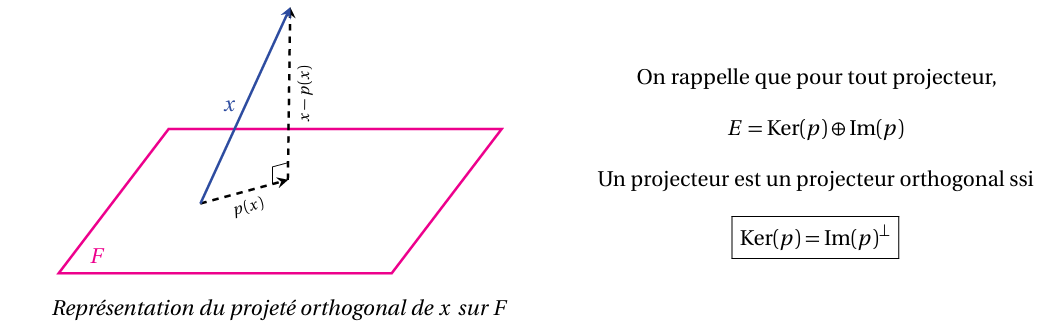
\includegraphics[width=1\linewidth]{image.png}
}
\Thm{Propriétés du projecteur orthogonal}{
En notant $p$ la projection orthogonale sur $F$, sous-espace vectoriel de $E$ de dimension finie $n$:\\
\begin{itemize}
    \item Si $x \in E$, $p(x)$ est entièrement caractérisé par : $p(x) \in F$ et $x - p(x) \in F^{\perp}$.
    \item Si $(e_1, \dots, e_n)$ est une base orthonormale de $F$, alors $p(x) = \langle x , e_1 \rangle e_1 + \dots + \langle x , e_n \rangle e_n$.
    \item La distance de $x$ à $F$ est donnée par : $d(x, F) = \inf_{u \in F} \|x - u\| = \|x - p(x)\|$.
\end{itemize}
\vspace{0.5em}
}

\Thm{Représentation matricielle d'un endomorphisme dans une BON}{
    Soit $u \in \mathcal{L}(E)$ et $\mathcal{B} = (e_1, \dots, e_n)$ une base orthonormale de $E$.
    
    \begin{itemize}
        \item La matrice $M = \mathrm{Mat}_{\mathcal{B}}(u)$ s'écrit alors :
        \[ M = \big( \langle u(e_j) , e_i \rangle\big) \]
        \item De plus, $M^TM = \big( \langle u(e_j) , u(e_i) \rangle\big)$
    \end{itemize}
    
}

\Thm{Représentation des formes linéaires}{
Soit $(E, \langle \cdot | \cdot \rangle)$ un espace euclidien. \\Pour toute forme linéaire $\varphi$, il existe un unique vecteur $a \in E$ tel que :
    \[ \forall x \in E, \quad \varphi(x) = \langle x , a \rangle \]
}

\subsubsection{Adjoint d'un endomorphisme}

\Def{Adjoint d'un endomorphisme}{
Soit $u \in \mathcal{L}(E)$. Il existe un unique endomorphisme $u^*$ de $E$ tel que :
\[
\forall x, y \in E, \quad \langle u(x), y \rangle = \langle x, u^*(y) \rangle
\]
On appelle $u^*$ l'adjoint de $u$.
}

\Thm{Propriétés de l'Adjoint (Stabilité Noyau Matrice Composition Involution)}{
\begin{itemize}
    \item Si $F$ SEV de $E$ : \quad\[u(F) \subset F \implies u^*(F^\perp) \subset F^\perp\]
    \item Noyau et Image : \[\ker u^* = \mathrm{Im}u ^{\perp} \quad \text{ et } \quad \mathrm{Im}u^* = \ker u ^{\perp}\]
    \item Si $B$ BON de $E$: \quad\[\mathrm{Mat}_B(u^*) = \mathrm{Mat}_B(u)^T\]
    \item Composition :
        \[ (u \circ v)^* = v^* \circ u^* \]
    \item Involution : Le passage à l'adjoint est involutif,
        \[ (u^*)^* = u \]
\end{itemize}
}

\subsubsection{Endomorphisme orthogonaux (noté O(E))}

\Def{Caractérisation des isométries vectorielles (1 def. + 4 caract.)}{
\begin{align*}
u \in O(E) 
    &\ssi  \quad \forall x \in E, \quad \|u(x)\| = \|x\|\\
    &\ssi \quad \forall x, y \in E, \quad \langle u(x), u(y) \rangle = \langle x, y \rangle\\
    &\ssi \quad u^* \circ u = \mathrm{id}_E\\
    &\ssi \quad u(BON) = BON\\
    &\ssi \quad \text{matrice de u dans une BON est orthogonale}\\
\end{align*}
}

\Thm{Caractérisation des matrices orthogonales (1 def. + 2 caract.)}{
\begin{align*}
A \in O_n(\R)
    &\ssi  \quad A^TA =I_n\\
    &\ssi  \quad \text{Les lignes de A forment une BON}\\
    &\ssi  \quad \text{Les colonnes de A forment une BON}\\
\end{align*}
}

\Def{Groupe spécial orthogonal}{
\[SO_n(\R) = \{O\in O_n(\R) \,/\, \det(O)=1 \}\]
}

\Thm{Propriétés des isométries (Stabilité Déterminant Spectre)}{
\textit{Si :} $u \in O(E), A =mat_{BON}(u)$ \\
\textit{Alors :}
\[
\begin{aligned}
    &u(F) \subset F \implies u(F^\perp) \subset F^\perp \\
    &\det(A) = \pm 1\neq0 \quad \\
    &Sp_\R(A) \subset \{-1,1\}\\
    &Sp_\C(A) \subset \mathbb{U}
\end{aligned}
\]
}

\Thm{Stabilité d'une droite ou d' un plan par un endomorphisme réel}{
Tout endomorphisme d'un espace de dimension finie admet au moins une droite ou un plan stable.


}

\Thm{Réduction des isométries}{
Soit $u \in O(E)$. $\exists B \text{ BON de E}$ tq :
\[
\left(
\begin{array}{cccccc}
I_p & 0 & 0 & \cdots & 0 \\
0 & -I_q & 0 & \cdots & 0\\
0 & 0 & R(\theta_1) & \\
\vdots & \vdots & & \ddots \\
0 & 0 & & & R(\theta_r)\\
\end{array}
\right)
\]
Pour $p + q + 2r = \dim(E)$, et $R$ des matrices de rotation de taille 2. ($\theta_i \not\equiv 0 \; [\pi]$) 
}

\Def{Symétrie orthogonale}{
\centering Une symétrie orthogonale à $F$ est la symétrie par rapport à $F$ //$^\text{ment}$ à $F^\perp$.\\
Si $F$ est un hyperplan de $E$, on parle de réflexion
}

\Thm{Caractérisation des symétries/projections orthogonale}{
\centering Une symétrie s $u$ est orthogonale $\ssi s\circ s = id,\; s\in O(E)$ .\\
\centering Une symétrie p $u$ est orthogonale $\ssi p\circ p = p,\; p\in O(E)$ .
}

\Thm{Caractérisation matricielle des symétries orthogonales}{
Une symétrie vectorielle est une symétrie orthogonale ssi sa matrice dans une base orthonormale est symétrique.\\

De plus, pour $M \in \mathcal{M}_n(\mathbb{R})$, deux des trois assertions suivantes impliquent la dernière :
    \begin{itemize}
        \item (i) $M^2 = I_n$
        \item (ii) $MM^\top = I_n$
        \item (iii) $M = M^\top$
    \end{itemize}
}

\Thm{Isométries du plan}{
    \begin{enumerate}
        \item $M \in \mathrm{O}_2(\mathbb{R}) \iff \exists \theta \in \mathbb{R}$ tel que $M = \begin{bmatrix} \cos \theta & \mp \sin \theta \\ \sin \theta & \pm \cos \theta \end{bmatrix}$
        \item $M \in \mathrm{SO}_2(\mathbb{R}) \iff \exists \theta \in \mathbb{R}$ tel que $M = \begin{bmatrix} \cos \theta & -\sin \theta \\ \sin \theta & \cos \theta \end{bmatrix}$
    \end{enumerate}
}

\subsubsection{Endormorphisme symétrique (noté $\mathcal{S}(E)$)}
\Def{Caractérisation des autoadjoints}{
\begin{align*}
u \in \mathcal{S}(E)
    &\ssi  \quad \forall x, y \in E, \quad \langle u(x), y \rangle = \langle x, u(y) \rangle \\
    &\ssi \quad \text{matrice de u dans une BON est symétrique ($A^T = A$)}\\
\end{align*}
}



\Thm{Stabilité de l’autoadjoint}{
\[u(F) \subset F \implies u(F^\perp) \subset F^\perp\]
}

\Thm{Orthogonalité de 2 espaces propres d'une symétrie}{
\centering Les espaces propres d'une symétrie sont orthogonaux
}

\Thm{Spectral}{
Si $u\in \mathcal{S}(E)$\\
\[u \text{ diagonalisable dans une BON de vecteurs propres et } E=\!\!\!\overset{\perp}{\bigoplus_{\lambda \in Sp(u)}} \!\!\!E_\lambda(u)\]

Si $A\in \mathcal{S}_n(\R)$\\
\[A \text{ diagonalisable et } A = PDP^T \text{  (où $P\in O_n(\R)$)}\]
}

\Thm{Caractérisation des projections orthogonale}{
\centering Une projection $p$ est une projection orthogonale $\ssi p\circ p = p,\; p\in S(E)$ .
}

\Def{Endomorphisme autoadjoint positif}{
Soit \textbf{$u \in S(E)$}. Les assertions suivantes sont équivalentes :
\begin{align*}
    (i) & \quad \forall x \in E, \quad \langle u(x), x \rangle \geq 0 \\
    (ii) & \quad Sp(u) \subset \mathbb{R}^+ \\
\end{align*}
}

\section{Exponentielle d'une Matrice}
\Def{Exponentielle d'un endomorphisme}{
Soit $u\in \mathcal{L}(E)$:
\[e^u = \sum_{k=0}^{+\infty}\frac{u^n}{n!}\]
et:
\[u\longmapsto e^u \text{ est continue}\]
}
\Thm{$\exp(u+v)$}{
Si $u,v$ commutent:
\[e^{u+v} = e^u\circ e^v\]
}
\Thm{L'inverse d'une exponentielle}{
\[e^u \in GL(E) \qquad e^{-u} = (e^u)^{-1}\]
}
\Thm{Dérivation}{
\[\varphi : t\longmapsto\exp(tA) \in D^1(\R) \quad \text{et} \quad \varphi'(t) = A \varphi(t)\]
}

\section{Groupes}
\subsubsection{Généralités}
\Thm{Caractérisation des sous groupes}{
\[H \text{ \ssgp{} }(G,\cdot) \ssi \leftaccolade{
 H\subset G\\
 e_G \in H\\
 \forall x,y \in H: xy^{-1}\in H \quad (\text{ou }x-y\in H)  
}\]
}

\Thm{Sous groupes de $\Z$}{
\[\text{Les sous groupes de $\Z$ sont les $n\Z$} \quad (n\in \N)\]
}
\Thm{Intersection de sous groupe}{
\[\text{Une intersection d'une famille de sous groupe est un sous groupe}\]
}

\Def{Groupe produit}{
    Soient $(G_1,\star_1),\dots,(G_n,\star_n)$ des groupes d'éléments neutres $e_1,\dots,e_n$.\\
    Pour tout $x = (x_1,\dots,x_n) \in G_1 \times\dots\times G_n$ et $y = (y_1,\dots,y_n) \in G_1\times \dots \times G_n$, on pose :
    $$x \star y = (x_1 \star_1 y_1,\dots, x_n \star_n y_n)$$\\
    Alors $G_1 \times\dots \times G_n$ est un groupe, appelé groupe produit, d'élément neutre $(e_1,\dots,e_n)$.
}

\subsubsection{Équivalence selon un sous-groupe}
\Def{Relation d'équivalence à gauche}{
Soit $(G,\star)$ un groupe et $H$ un sous-groupe de $G$. \\On note $\mathcal R$ la relation définie sur $G$ par :
$$\forall (x,y) \in G^2 \quad x \mathcal{R} y \quad x^{-1}y \in H$$
Alors $\mathcal R$ définit une relation d'équivalence sur $G$ 
\\\textbf{La classe d'équivalence de $x \in G$ est $\overline{x} = xH$}.
}

\Thm{de Lagrange (HP)}{
Soit H ss gpe de G \textbf{fini}:
\[\card(H) |\card(G) \]

\textit{Si $G$ est de cardinal $p$ premier, $G$ admet deux sous-groupes : $\{e\}$ et $G$.}
}

\newpage
\subsubsection{Groupe quotient \textbf{(Groupe abélien fini)}}
Soit $(G,+)$ un \textbf{groupe abélien fini}, $H$ un sous-groupe de $G$ et $\cal R$ la relation d'équivalence selon $H$.

\Def{Ensemble quotient}{
L'\textbf{ensemble des classes d'équivalence} est appelé ensemble quotient et noté $G/\cal R$.
}

\Thm{Addition sur un ensemble quotient}{
    Pour $(x,y) \in G^2$ on pose :
    $$\overline{x}\oplus\overline{y}=\overline{x+y}$$.
    Alors $ \oplus$ est une LCI sur $G/ \cal R$.
}

\subsubsection{Morphisme de groupe}
\Def{Morphisme de groupe}{
On appelle morphisme de groupes entre $(G,+)$ et $(H,*)$ toute application $f:G\to H$ telle que :
\[\forall x,y\in G: f(x+y) = f(x)*f(y)\]
\textit{Le noyau et l'image sont des sous groupe}
}

\Thm{Si $f$ isomorphisme}{
Si $f$ isomorphisme alors $f^{-1}$ est un isomorphisme
}

\Thm{Propriétés de morphisme}{
Pour $f:G\to G'$ un morphisme:
\[f(e) = e' \text{ et } f(x)^{-1}=f(x^{-1})\]
\[H \text{ ssgpe de }G \implies f(H) \text{ ssgpe de }G'\]
\[Im(f) = f(G) \text{ et } ker(f)=f^{-1}(\{e'\})\]
\[f \text{ surjective} \ssi Imf=G'\]
\[f \text{ injective} \ssi kerf=\{e\}\]
}

\Thm{Isomorphisme (HP)}{
($G$,+) abélien et ($G'$, $\cdot$) gpe\\
$f : G\to G'$ un morphisme
\[G/kerf \text{ est isomorphe à } Imf\]
}

\subsubsection{Génération de groupes}

\Def{Groupe engendré par une partie}{
Soit $A\subset G$\\
On note $(A)$ l'\textbf{intersection} de tous \textbf{les sous groupes} de $G$ \textbf{contenant A}\\
Si $(A) = G$ alors $A$\textbf{ est une partie génératrice de} $G$\\
\textit{Cas particulier important:}
\[G = (a) = \{ a^k / k \in \Z\}\]
}

\Def{Groupe monogène et cyclique}{
    Un groupe est dit \textbf{monogène} s'il est engendré par un unique élément.\\
    Un groupe est dit \textbf{cyclique} s'il est monogène et fini.
}

\Thm{Classification des groupes monogènes}{
    Un groupe monogène est isomorphe à :
    \begin{itemize}
        \item $(\Z,+)$ s'il est infini
        \item $(\Z/n\Z,+)$ s'il est fini et de cardinal $n$
    \end{itemize}
}

\Thm{Générateur de $\Z/n\Z$}{
    Soit $n \in \N^*$ et $k \in [|1,n|]$.\\
    \[(\overline k) = \Z /n\Z \ssi k\land n = 1\]
}

\subsubsection{Ordre d'un élément}

\Def{Ordre d'un élement}{
Pour $a \in G$: 
\[\omega(a)=\min\{k\in \N^*/ a^k=e\} \cup\{ +\infty\}\]
}

\Thm{Caractérisation cyclique}{
Pour $G$ un groupe fini de cardinal $n$,
$$G \text{ cyclique} \ssi \exists a\in G :\omega(a)=n$$
}

\Thm{Prop 3 étoiles}{
Soit G gpe, $a$ d'ordre fini $p$ alors : 
\[\forall q\in \Z :\quad a^q=e\ssi p|q\]
\textit{Le seul moyen que $a^q =e$ est que $p$ soit plus petit (au sens de la division) que $q$ car $a^p=e$}\\
et:
\[\text{Si}, \quad \exists p\in\N^*,\forall q\in \Z :\;  a^q=e\ssi p|q \:\quad \text{ alors } \:\omega(a) =p  \]
\textit{L'équivalence plus haut caractérise l'ordre de $a$}
}

\Thm{Caractérisations équivalentes de "a engendre G"}{
Soit $(G,\cdot)$ un groupe fini cyclique d'ordre $n$, et soit $a\in G$. Alors
\begin{align*}
a \text{ est générateur de } G
&\iff \operatorname{ord}(a)=n \\
&\iff \forall k\in\mathbb{Z},\; a^k=e \Longleftrightarrow n\mid k \\
&\iff \forall p\mid n,\; p \text{ premier},\; a^{n/p}\neq e.
\end{align*}

De plus (\textit{hors programme}), si $G=\langle a\rangle$ pour $k\in\mathbb{Z}$, alors
\[
a^k \text{ est générateur de } G \iff k\land n=1.
\]

\textit{Ce dernier point ce montre avec la formule $\omega(a^k)$}
}

\Thm{L'ordre divise l'ordre (Lagrange faible)}{
\[\text{L’ordre d’un élément d’un groupe fini divise le cardinal du groupe}\]
}

\Thm{$\omega(a^k) ?$ (HP)}{
\[\forall k \in \Z:  \omega(a^k)=\frac{p}{p\wedge k}\]
où $p = \omega(a)$
}

\Thm{$a^k$ générateur ssi ? (HP)}{
Soit \(k \in \Z\) tel que $G=(a)$: 
\[a^k \text{ générateur de }G \ssi k\wedge n=1 \]
}




\subsubsection{Groupe symétrique}
\Def{Représentation des permutations}{
Soit $\sigma \in S_n$, on représente la permutation $\sigma$ :
\[
\sigma = \begin{pmatrix}
1 & 2 & \cdots &n \\
\sigma(1) & \sigma(1) & \cdots & \sigma(n)
\end{pmatrix}
\]
}
\Def{Support d'une permutation}{
On note le support de la permutation $\sigma\in S_n$:
\[\mathrm{Supp(\sigma)} = \{k\in[|1,n|] \, /\, \sigma(k)\neq k\}\]
}
\Thm{Commuter 2 permutations}{
\[\text{Deux permutations de $[|1,n|]$ à support disjoints commutent}\]
}

\Def{$p$-cycle et transpositions}{
Un $p$-\textbf{cycle} est une permutation $\sigma \in S_n$ telle que \(\exists\,a_1,a_2,\dots,a_p \in[|1,n|]\):
\[\sigma(a_1) = a_2 \quad \sigma(a_2) = a_3\quad \dots \quad \sigma(a_{p-1}) =a_p \quad \sigma(a_p) = a_1\]
\[\forall k \in[|1,n|]\textbackslash{\{a_1,\dots,a_p\}}: \sigma(k)=k\]

On note $\sigma = (a_1 \!\quad \!a_2 \!\quad \!\dots\! \quad \!a_p)$\\
Une \textbf{transposition} est un cycle de longueur 2, noté $\tau_{ij}$
}

\Thm{Décomposition de permutation}{
\[\text{Toute permutation peut se décomposer en un produit de cycles à support disjoints}\]
}

\Thm{Décomposition de permutation 2}{
\[\text{Tout permutation peut se décomposer en un produit de transposition}\]
}

\Def{Signature d'une permutation}{
\[\varepsilon(\sigma) = (-1)^m = \prod_{1\leq i<j\leq n} \frac{\sigma(i)-\sigma(j)}{i-j}\]
où \(m = \card\{(i,j)/ \;i<j\, \text{  et } \, \sigma(i)>\sigma(j)\} =\) "nombre d'inversion entre 2 éléments"

\textit{La signature d'un $p$-cycle est : $\varepsilon(\sigma) = (-1)^{p-1}$}
}

\section{Anneaux et corps}
\Thm{Caractérisation des sous-anneaux}{
Soit $(A,+,\times)$ un anneau. $B \subset A$ est un sous-anneau de $A$ si et seulement si $1_A \in B$ et :
\[
\forall x,y \in B,\qquad x-y \in B \qquad \text{et} \qquad x\times y \in B
\]
}
\Def{Corps}{
Un \textbf{corps} $K$ est un anneaux (commutatif \textit{seulement pour le programme}) tel que :\\
Tout élément hormis $0_K$ est inversible
}

\Def{Caractérisation des sous-corps}{
Soit $(\mathbb{K},+,\times)$ un corps. $\mathbb{K}' \subset \mathbb{K}$ est un sous-corps de $\mathbb{K}$ si et seulement si :
\[
\forall x,y \in \mathbb{K}' \times \mathbb{K}'^{*},\qquad x-y \in \mathbb{K}' \qquad \text{et} \qquad x\times y^{-1} \in \mathbb{K}'
\]
}

\subsubsection{Morphismes de corps et d'anneaux}
\Def{Morphisme d'anneaux}{
Soient $A$ et $B$ deux anneaux. On appelle morphisme de $A$ dans $B$ toute application $\phi : A \to B$ qui vérifie :
\[
\text{(i)}\ \forall x,y \in A,\ \phi(x+y)=\phi(x)+\phi(y)
\qquad
\text{(ii)}\ \forall x,y \in A,\ \phi(x\times y)=\phi(x)\times\phi(y)
\qquad
\text{(iii)}\ \phi(1_A)=1_B
\]

\textit{Un morphisme de corps possède la même definition, c'est en particulier un morphisme de groupe}
}

\subsubsection{Idéal d'un anneau commutatif}
\Def{Idéal d'un anneau commutatif}{
Soit $(A,+,\times)$ un anneau commutatif. On appelle idéal de $A$ toute partie $I$ de $A$ telle que :
\(\text{(i)}\ (I,+)\text{ est un sous-groupe de }(A,+)\)\\
\(
\text{(ii)}\ I\text{ fortement stable par }A :
\qquad \forall a\in A,\ aI\subset I.
\)
}
\Def{Idéal principal}{
Soit $x$ un élément d’un anneau commutatif $A$. \\
$(x)=xA$ est le plus petit idéal de A contenant $x$\\
On dit que \textbf{$(x)$ est l'idéal principal de $A$}

\medskip

\textit{On rappelle que l’on note $a\mid b$ pour $a,b$ éléments d’un anneau commutatif s’il existe $c\in A$ tel que $b=c\times a$.
Alors,
\[
x\mid y \iff yA\subset xA \iff (y)\subset (x)
\]}
}

\Thm{Opération sur les idéaux}{
Soient $I_1$ et $I_2$ deux idéaux d’un anneau commutatif $A$. Alors,
\begin{itemize}
    \item $I_1\cap I_2$ est un idéal de $A$ ;
    \item $I_1+I_2=\{x_1+x_2 \mid (x_1,x_2)\in I_1\times I_2\}$ est un idéal de $A$.
\end{itemize}
}

\Def{Caractéristique d'un anneau (HP)}{
Soit $A$ un anneau unitaire. Soit $f : n\in\Z \longmapsto n1_A$\\
Si $\ker f = \{0\}$ : $A$ est de \textit{caractéristique} $0$\\
Si $\ker f \neq \{0\}$ : $\ker f$ étant un idéal de $\Z$, on note la \textit{caractéristique} de $A$, $c\in \N^*$: $c\Z = \ker f$

\textit{On a : $n1_A=0\ssi c|n$}
}

\section{Arithmétique}
\subsubsection{Arithmétique dans $\Z$}
\Thm{Les idéaux de $\Z$}{Les idéaux de $\Z$ sont les $n\Z$}
\Thm{Relation idéaux de $\Z$ et pgcd ppcm}{
Soit $a,b\in \Z^*$:\\
$\quad a\Z+b\Z = (a\land b)\Z$\\
$\quad a\Z\cap b\Z = (a\vee b)\Z$
}
\textit{Il y a aussi le Lemme de Gauss et le Théorème de Bezout}

\Thm{Structure d'anneau de $\Z/n\Z$}{
$(\mathbb{Z}/n\mathbb{Z},+,\times)$ est un anneau.
}
\Thm{Meilleur structure de $\Z/p\Z$}{
Les assertions suivantes sont équivalentes :
\begin{enumerate}
    \item[(i)] $\mathbb{Z}/p\mathbb{Z}$ est un corps.
    \item[(ii)] $\mathbb{Z}/p\mathbb{Z}$ est un anneau intègre.
    \item[(iii)] $p$ est premier.
\end{enumerate}
}
\Thm{Inversible de $\Z/n\Z$}{
L’élément $\overline{k}$ est inversible dans l’anneau $\mathbb{Z}/n\mathbb{Z} \ssi k \wedge n = 1$.\\
\textit{La preuve nous fournit une méthode pour trouver l’inverse d’un élément de $\Z/n\Z$
}
}

\subsubsection{Indicatrice d'Euler}

\Def{Indicatrice d'Euler}{
Pour $n\in\mathbb{N}^*$, on pose
\[
\varphi(n)=\operatorname{card}\{k\in\llbracket 1,n\rrbracket \mid k\wedge n=1\}.
\]
\textit{La fonction $\varphi$ est appelée indicatrice d’Euler.
$\varphi(n)$ représente :
\begin{itemize}
    \item le nombre d’entiers inférieurs à $n$ et premiers avec $n$ ;
    \item le nombre d’éléments inversibles de l’anneau $\mathbb{Z}/n\mathbb{Z}$ ;
\end{itemize}}
}

\Thm{Lemme chinois}{
Si $m$ et $n$ sont deux entiers premiers entre eux,
\[
\mathbb{Z}/mn\mathbb{Z}\ \text{est isomorphe à }\ \mathbb{Z}/m\mathbb{Z}\times \mathbb{Z}/n\mathbb{Z}.
\]
}

\Thm{Propriété indicatrice d'Euler (conséquence du lemme chinois)}{
Soient $m,n\in\mathbb{N}^*$. Si $m\wedge n=1$, \(\varphi(mn)=\varphi(m)\varphi(n)\).
}

\Thm{{$\varphi(p^k)$, déduire l'expression de $\varphi(n)$}}{
Soit $p\in\mathbb{P}$ et $k\in\N^*$ :
\[
\varphi(p^k)=p^{k-1}(p-1)
\]
Soit $n\in\N^*$, avec
\[
n=p_1^{\alpha_1}\cdots p_m^{\alpha_m}
\]
où les $p_i$ sont deux à deux distincts et les $\alpha_i\in\N^*$.
Alors
\[
\varphi(n)=\prod_{i=1}^m p_i^{\alpha_i-1}(p_i-1)
= n\prod_{i=1}^m \left(1-\frac{1}{p_i}\right)
\]
}
\Thm{D'Euler}{
Soient $a\in\mathbb{Z}$ et $n\in\mathbb{N}\setminus\{0,1\}$. Si $a\wedge n=1$, alors
\[
a^{\varphi(n)}\equiv 1 \pmod n.
\]

$\varphi(n)$\textit{ est le cardinal du groupe des inversibles }\\
\textit{Si } $a\wedge n=1,\ \overline{a}$\textit{ est un élément de ce groupe, donc :}\\
$\omega(a)|card((\Z/n\Z)^*)=\varphi(n)$ \textit{ et }
$\overline{a}^{\,\varphi(n)}=\overline{1}
\iff
a^{\varphi(n)}\equiv 1 \quad[n]$
}

\subsubsection{Arithmétique dans K[X]}
Soit $\K$ un sous-corps de $\C$.

\Thm{Idéaux de l'anneau des polynômes} {
Tout idéal de $\K[X]$ est de la forme
\[
(P)=P\K[X]=\{PQ \mid Q\in \K[X]\},
\qquad \text{où } P\in \K[X].
\]
}

\Def{Polynômes irréductible}{
\[P\in\K[X] \text{ non constant, irréductible} \ssi P \text{ n'est divisible divisible que par 1 et $P$}\]
\textit{à une constante mult. près}
}

\Thm{Existence d'un polynôme irréductible}{
Tout polynôme non constant $P\in\K[X]$ admet un diviseur irréductible.
}

\Thm{D'euclide}{
Soit $A$ et $B$ deux polynômes de $\K[X]$ et $P$ un polynôme irréductible. \\
Si $P|AB$, $P|A$ ou $P|B$.
}

\chapter{Probabilités}
\section{Dénombrement}
\Def{p-uplet arrangement permutation combinaison}{
Pour $\mathrm{Card}(\Omega) = n$ :
\begin{itemize}
    \item \textbf{p-uplet ou p-liste de $\Omega$.}\\
    C’est une famille de $p$ éléments de $\Omega$. Les éléments peuvent se répéter.

    \item \textbf{Arrangement de $p$ éléments de $\Omega$.}\\
    C’est un p-uplet formé de $p$ éléments \emph{distincts} de $\Omega$. 

    \item \textbf{Permutation de $\Omega$.}\\
    C’est un p-uplet formé de $n$ éléments \emph{distincts} de $\Omega$.

    \item \textbf{Combinaison de $p$ éléments de $\Omega$.}\\
    C’est un sous-ensemble de $\Omega$ contenant $p$ éléments.
\end{itemize}
}
\Thm{Nombre de p-uplet arrangement permutation combinaison}{
Pour $\mathrm{Card}(\Omega) = n$ :

\begin{itemize}
    \item Il y a \(n^p\) \(p\)-listes de \(\Omega\).
    \item Il y a \(\displaystyle \frac{n!}{(n-p)!}\) arrangements de \(p\) éléments de \(\Omega\).
    \item Il y a \(n!\) permutations de \(\Omega\).
    \item Il y a \(\displaystyle \binom{n}{p}\) combinaisons de \(p\) éléments de \(\Omega\).
\end{itemize}
}

\section{Probabilités discrètes}

\Def{Tribu}{
Une tribu sur \(\Omega\) est une partie \(\mathcal{A}\) de \(\mathcal{P}(\Omega)\) qui vérifie :
\begin{enumerate}
    \item \(\Omega \in \mathcal{A}\) ;
    \item Si \(A \in \mathcal{A}\) alors \(\overline{A} \in \mathcal{A}\) ;
    \item Si \((A_n)_{n \in \mathbb{N}} \in \mathcal{A}^{\mathbb{N}}\), alors \(\displaystyle \bigcup_{n=0}^{\infty} A_n \in \mathcal{A}\).
\end{enumerate}
}

\Def{Système complet d'évenements}{
\[(A_1, ...., A_n) \text{ SCE } \ssi \bigsqcup_{k=1}^n A_i = \Omega\]
}

\Def{Probabilité}{
%Cov(X,Y) = 0 \ssi X,y indep
On appelle \emph{probabilité} sur \((\Omega,\mathcal{A})\) toute application
\(P : \mathcal{A} \to [0,1]\) vérifiant :
\begin{enumerate}
    \item \(P(\Omega) = 1\).
    \item  \(\forall (A_n)_{n\in\mathbb{N}} \in \mathcal{A} :\)    \[
        P\!\Bigl(\bigsqcup_{n=0}^{+\infty} A_n\Bigr) 
        = \sum_{n=0}^{+\infty} P\bigl(A_n\bigr)
    \]
\end{enumerate}
}

\Thm{Propriétés usuelles d'une probabilité}{
Soient \((\Omega, \mathcal{A}, P)\) un espace probabilisé et \(A, B \in \mathcal{A}\).
\begin{itemize}
    \item $P(A\textbackslash B) = P(A) - P(A\cap B)$
    \item \(P(\overline{A}) = 1 - P(A).\)
    \item Si \(A \subset B\) alors \(P(A) \le P(B).\)
    \item \(P(A \cup B) = P(A) + P(B) - P(A \cap B).\)
\end{itemize}
}

\Def{Indépendance}{
$(A_i)_{i\in I}$ sont (mutuellement) indépendants si:
\[
\forall J\subset I \text{ finie}: 
P\!\Bigl(\bigcap_{j \in J} A_j\Bigr) \;=\; \prod_{j \in J} P(A_j)
\]
}

\Thm{Distribution de probabilités}{
    \[\sum_{\omega\in\Omega} P({\omega}) = P(\Omega) = 1\]
}

\Thm{Continuité croissante}{
Si \((A_n)_{n \in \mathbb{N}}\) est une suite croissante d'événements, alors :
\[
 \lim_{n \to +\infty} P(A_n) = P\!\Bigl(\bigcup_{n=0}^{+\infty} A_n\Bigr)
\]
}

\Thm{Union et intersection d'évenements néglibeable ou presque sûr}{
\[\bigcup_{\text{au plus den}} \text{evts négligable} = \text{evt négligable}\]
\[\bigcap_{\text{au plus den}} \text{evts presque sûr} = \text{evt presque sûr}\]
}

\Thm{Sous additivité}{
    \[
        P\!\Bigl(\bigcup_{k=0}^{n} A_k\Bigr) \;\le\; \sum_{k=0}^{n} P(A_k).
    \]
    \textit{De même pour une union infinie sur la série converge}
}

\Thm{Formule des probabilités composées}{
\[
P(\bigcap_{k=0}^nA_k)
= P(A_1)\, P_{A_1}(A_2) \times \cdots \times P_{A_1 \cap \cdots \cap A_{n-1}}(A_n).
\]
}

\Thm{Formule des probabilités totales}{
Soit \((A_n)_{n \in \mathbb{N}}\) un SCE.
\[
P(B) \;=\; \sum_{n=0}^{\infty} P\bigl(B \cap A_n\bigr)
\;=\; \sum_{n=0}^{\infty} P_ {A_n}\bigl(B\bigr)\,P(A_n).
\]
}

\Thm{Formule de Bayes}{
\[
P(A \mid B) \;=\; \frac{P(A)}{P(B)} \;\times\; P(B \mid A).
\]
}

\section{Variables aléatoires}
\Def{Loi conjointe et lois marginales}{
\begin{itemize}
    \item La loi conjointe de \(X\) et de \(Y\) est la loi de \((X,Y)\). 
          \textit{(donnée par \(P(X = x \cap Y = y)\))}
    \item Les lois marginales de \((X,Y)\) sont celles de \(X\) et de \(Y\).
\end{itemize}
}

\Def{Espérance}{
\(X\) est dite d'espérance finie si la famille \(\bigl(x\,P(X=x)\bigr)_{x \in X(\Omega)}\) 
est sommable.\\
\[
\mathbb{E}(X) \;=\; \sum_{x \in X(\Omega)} x\,P(X=x).
\]
\\
Si \(X\) est à valeurs dans \(\mathbb{N}\) et d'espérance finie, alors :
\[\mathbb{E}(X) \;=\; \sum_{n=0}^{+\infty} P\bigl(X > n\bigr).\]
}

\Thm{Linéarité de l'espérance}{
    \[E(\lambda X + Y) = \lambda E(X) + E(Y)\]
}

\Thm{Du transfert}{
\[
X\in L^1 : \mathbb{E}(f(X)) \;=\; \sum_{x \in X(\Omega)} f(x)\,P(X=x).
\]
}

\Thm{Comparaison $L^p$}{
\centering Si \(\lvert X \rvert \le Y\) et \(Y \in L^p\), alors \(X \in L^p\).
}

\Thm{Espérance et indépendance}{
Pour \(X, Y \in L^1\) indépendantes: 
\(XY \in L^1\) 
\[
\mathbb{E}(XY)\;=\; \mathbb{E}(X) \,\mathbb{E}(Y).
\]
\textit{Vrai pour un produit de $n$ lois}
}

\Thm{Formule de Kœnig-Huygens}{
Pour \(X \in L^2\)
\[
V(X) \;=\; \mathbb{E}(X^2) \;-\;  \mathbb{E}(X)^2.
\]
\textit{Cas particulier :} $V(aX+b) =a^2V(X)$
}

\Thm{Formule de Kœnig-Huygens pour la covariance}{
Pour \(X,Y \in L^2\)
\[
Cov(X,Y) = E(XY)-E(X)E(Y)
\]
}

\Thm{Variance d'une somme}{
\[V(\sum_{i=0}^nX_i )= \sum_{i=0}^nV(X_i) + 2\sum_{1\le i< j\le n} Cov(Xi,Xj)\]
Si indep : 
\[V(\sum_{i=0}^nX_i)= \sum_{i=0}^nV(X_i)\]
}

\Def{Lois équivalentes}{
    \[X\sim Y \overset{def}{\ssi} P_X = P_Y\]
}

\Thm{Fonction appliqué à des lois équivalentes}{
\[X \sim Y \implies f(X) \sim f(Y)\]
}

\Thm{Lemme des coalitions}{
Soit $(X_1,X_2,...,X_n)$ des v.a.d. et indépendantes.

Les variables $f(X_1, \ldots, X_k)$ et $g(X_{k+1}, \ldots, X_n)$ sont indépendantes.
}
\Thm{Inégalité de Cauchy-Schwartz}{
Pour $X,Y\in L^2$
    \[|E(XY)|\le\sqrt{E(X^2)E(Y^2)}\]
}
\Thm{Inégalité de Markov}{
Pour $X\in L^1$
    \[\forall a>0 :P(|X| \geq a) \leq \frac{E(|X|)}{a}\]
 }
\Thm{Inégalité de Bienaymé-Tchebychev}{
Pour $X\in L^2$
    \[\forall \varepsilon>0 :P(|X-E(X)| \geq \varepsilon) \leq \frac{V(X)}{\varepsilon^2}\]
 }

\Thm{Loi faible des grands nombres}{
Pour $(X_n)_{n\in\N}$ des variables indépendantes et identiquement distribuées
\[\forall \varepsilon>0 : P(|\frac{S_n}{n}-E(X)|\ge\varepsilon)\xrightarrow [n\to+\infty]{} 0\]
}

\Def{Fonctions génératrices}{
Pour $X$ à valeurs dans $\N$ et $X_i$ indépendantes
\[G_X \text{ fonction génératrice de } X \overset{def}\ssi G_X : t\mapsto E(t^X) = \sum_{n=0}^{+\infty}P(X=n)t^n\]
}
\Thm{Caractérisation de fonctions génératrices}{
\[G_X = G_Y \ssi X\sim Y\]
}
\Thm{Continuité et Dérivabilité de fonctions génératrices}{
\[G_X \text{ est } C^0 \text{ sur [-1,1]} \quad \text{ et }\quad G_X \text{ est } C^\infty \text{ sur ]-1,1[}\]
}
\Thm{Formules de fonctions génératrices}{
\[\forall n \in \N : P(X=n) = \frac{G_X^{(n)}(0)}{n!} \quad \text{ et }\quad G_{\sum_{i=0}^nX_i} = \prod_{i=0}^nG_{X_i} \text{ avec $X_i$ indep}\]
\[\text{Formule de Wald}: (X_n)_{n\in \N}\;iid \implies G_{S_N}=G_N\circ G_{X_1}\]
}


\end{document}

